\documentclass[12pt]{extarticle}

\usepackage{geometry}
\geometry{
a4paper,
total={170mm,257mm},
left=20mm,
top=20mm,
headheight=12pt
}

\usepackage[parfill]{parskip} % Activate to begin paragraphs with an empty line rather than an indent
\usepackage{graphicx}
\usepackage{amsmath, amssymb, amsthm}
\usepackage[font=small,labelfont=bf]{caption, subcaption}
\usepackage{setspace}\onehalfspacing
\usepackage[loose,nice]{units}
\usepackage{array}
\usepackage[super]{nth}
\usepackage{graphicx}
\usepackage{float}
\usepackage{varioref}
\usepackage[unicode=true,colorlinks=true,urlcolor=blue,citecolor=black,linkcolor=black]{hyperref}
\usepackage{cleveref}
\usepackage{subcaption}
\usepackage{mathtools}
\usepackage[all]{nowidow}
\usepackage{wrapfig}
\usepackage{pdfpages}
\usepackage{authblk}
\usepackage[utf8x]{inputenc}
\usepackage[english]{babel}
% appendix
\usepackage[title,page]{appendix}
\usepackage{chngcntr}
% unbreakable dashes
\usepackage[shortcuts]{extdash}
% footnotes
\renewcommand{\thefootnote}{\fnsymbol{footnote}}

% less space before sections 
% \titlespacing*{<command>}{<left>}{<before-sep>}{<after-sep>}
\usepackage{titlesec}
\titlespacing*{\section}
{0pt}{2ex plus 1ex minus .2ex}{2ex plus .2ex}
\titlespacing*{\subsection}
{0pt}{1ex plus 1ex minus .2ex}{1ex plus .2ex}
\titlespacing*{\paragraph}
{0pt}{1ex plus 1ex minus .2ex}{1ex plus .2ex}

%SetFonts
% newtxtext+newtxmath
\usepackage{newtxtext} %loads helv for ss, txtt for tt
\usepackage{amsmath}
\usepackage[bigdelims]{newtxmath}
\usepackage[T1]{fontenc}
\usepackage{textcomp}
%SetFonts

% line numbers
\usepackage[displaymath, mathlines]{lineno}
 \renewcommand\linenumberfont{\normalfont\small\sffamily}
%%%%\linenumbers
\modulolinenumbers[2]

% Supplementary
\newcommand{\beginsupplement}{%
      	\setcounter{table}{0}
        \renewcommand{\thetable}{S\arabic{table}}%
        \setcounter{figure}{0}
        \renewcommand{\thefigure}{S\arabic{figure}}%
        \setcounter{equation}{0}
        \renewcommand{\theequation}{A\arabic{equation}}%
}

% NatBib
%\usepackage[super,comma]{natbib}
\usepackage[round,colon,authoryear]{natbib}
%\use-package[numbers,super,sort&compress]{natbib}
\renewcommand{\bibsection}{}
%\renewcommand{\bibfont}{\small}

% math stuff
\DeclareMathOperator*{\E}{{\rm I\kern-.3em E}}
\newcommand*{\tr}{^\intercal}
\let\vec\mathbf
\newcommand{\matrx}[1]{{\left[ \stackrel{}{#1}\right]}}
\newcommand{\diag}[1]{\mbox{diag}\matrx{#1}}
\newcommand{\goesto}{\rightarrow}
\newcommand{\dspfrac}[2]{\frac{\displaystyle #1}{\displaystyle #2} }
\newtheorem{theorem}{Theorem}
\newtheorem{corollary}{Corollary}
\newtheorem{lemma}{Lemma}
\newtheorem{remark}{Remark}
\newtheorem{result}{Result}
\renewcommand\qedsymbol{} % no square at end of proof
\newcommand{\cl}{\mathbf{L}}
\newcommand{\cj}{\mathbf{J}}
\newcommand{\ci}{I}

% line numbers
\usepackage[displaymath, mathlines]{lineno}
\renewcommand\linenumberfont{\normalfont\small\sffamily}
\linenumbers
\modulolinenumbers[2]


% Title page
\title{Prestige bias in cultural evolutionary dynamics}
% Authors
\renewcommand\Affilfont{\small}

\author[1]{Saar Egozi}
\author[2,3,$\dagger$]{Yoav Ram}

\affil[1]{School of Computer Science, Reichman University, Herzliya, Israel}
\affil[3]{School of Zoology, Faculty of Life Sciences, Tel Aviv University, Tel Aviv, Israel}
\affil[3]{Sagol School of Neuroscience, Tel Aviv University, Tel Aviv, Israel}
%\affil[*]{These authors contributed equally to this work}
\affil[$\dagger$]{Corresponding author: yoav@yoavram.com}


\begin{document}
\maketitle

\begin{abstract}
A common bias in cultural transmission is to copy whoever appears more successful. This success bias only depends on the performance of the role-model.
Because success may be difficult to estimate, it has been suggested that individuals may indirectly estimate success by using prestige as a proxy for success. However, prestige can be defined in different ways: it can reflect performance in another, possibly related, task; but it can also reflect overall influence of the role-model, irrespective of performance.
Here, we model prestige bias as a combination of indirect success bias and influence bias, the latter meaning that the choice of a role-model depends on the number of individuals that have already copied from that role-model.
We analyze the effect of prestige on cultural evolutionary dynamics using mathematical analysis and stochastic simulations.
We find analytic approximations to the stochastic role-model choice process, which facilitate further mathematical analysis and reduce the computational complexity of simulations. We validate these approximations and demonstrate their robustness to model assumptions.
We also find approximations to the fixation probability and the fixation time of an invading cultural trait, in both constant and changing environments. 
These approximations are similar to Kimura's approximations for population-genetic models.
These similarities show that indirect success bias effectively plays the role of natural selection, whereas influence bias effectively plays the role of genetic drift.	
Influence bias also accelerates the evolutionary dynamics, as can be expected in a \emph{rich-getting-richer} process.
Our model extends the literature that describes and analyses cultural transmission, 
especially in human societies where social media is popular and thus influence bias may be expected. 
Further work is needed to test if this model could explain and predict various phenomena in cultural evolution.
\end{abstract}


\pagebreak


\section*{Introduction}

%\paragraph{Cultural transmission.}
In cultural transmission, individuals transmit cultural traits (i.e., behaviors, beliefs, norms) to one another, typically by learning and demonstrating \citep{transmissionVectorsBook}.
Examples for cultural traits in humans are norms, preferences, tools, ideas, and language, potentially transmitted verbally and/or by observations \citep{transmissionVectors}. 
Although cultural transmission is common in humans, it is also observed in other animals, e.g. chimpanzees \citep{chimpsPrestige, chimpsCopy}, dolphins and whales \citep{dolphins_whales}, elephants \citep{elepahntsRepo}, and even flies \citep{fliesPaper} and fish \citep{Truskanov2020}.

Cultural transmission may combine vertical transmission, in which parents transmit to their offspring; oblique transmission, in which adults (teachers, leaders, and even strangers) transmit to unrelated offspring; and horizontal transmission, in which peers from the same age cohort transmit to one another \citep{transmissionVectorsBook,transmissionVectors}.
It has been demonstrated that non-vertical cultural transmission can maintain maladaptive traits, which can be beneficial in changing environments \citep{changeEnv}. 

Transmission biases may cause a cultural trait to have a disproportionate probability to be transmitted compared to its frequency in the population. \textit{Success bias} occurs when individuals prefer to copy from role models that demonstrate success in some activity, such as fishing, growing yams, using medicinal plants \citep{fijian_social_bias}, or hunting \citep{Mesoudi2008}, and it can increase the probability of learning a successful trait \citep{Borofsky2022}. 
Indeed, in a tournament between learning strategies conducted by \citet{strategiesPaper}, most winner strategies included a mixture of success-biased social learning and individual learning, implying that success-biased learning is a good strategy, but that by itself it is not enough to best other strategies, even when success is measured accurately.

% TODO edit so that we focus on indirect success - aka prestige - and decompose it to content based - which we call success - and context based - which we call influence
\citet[Ch.~5]{evolutionBook} have suggested that the evaluation of success can be divided to three categories: \emph{direct bias}, \emph{indirect bias} and \emph{frequency-dependent bias}.
A direct bias occurs when one phenotype is more attractive than other phenotypes, and is evaluated by \emph{directly} testing the trait.
For example, an individual observing a ping-pong match can attempt the observed paddle grips to determine which grip is better.
A frequency-dependent bias occurs when the probability to copy a phenotype is higher or lower than the frequency of the phenotype among demonstrators. 
For example, suppose the common paddle grip is used by 60\% of the demonstrators; if the this grip is adopted by 80\% of copiers, then transmission is under positive frequency bias, also called \emph{conformity}; if it is adopted by 40\% of copiers, then transmission is under negative frequency bias, or \emph{non-conformity} \citep{conformism}. 
The effects of conformity and non-conformity on cultural evolution have been studied with both models \citep{anticonformity,Denton2021,conformity} and experiments \citep{negativeFrequency}.
An indirect bias occurs when an individual uses one phenotype to determine the attractiveness of another phenotype.
For example, an observer may copy the paddle grip of the ping-pong player who scored more points in the match, thus indirectly evaluating the grip by the points scored.
This, however, may cause mismatches between the copied trait and the rest of the cultural or genetic repertoire of the individual \citep{Kolodny2022}.
Furthermore, \citet[Ch. 8]{evolutionBook} have suggested that maladaptive traits may spread widely in a population if indirect biases are strong enough by a runaway process caused by a cultural equivalent of sexual selection \citep{sexualSelectionBook}.
For example, \citet{cooperation} have shown that helping behaviors can evolve due to horizontal transmission bias even without any benefit to the recipient, or when the benefit is much larger than the cost.

\citet{fijian_social_bias} have studied such indirect success biases, which they call cross-domain success bias or \emph{prestige bias} (e.g., great fishermen may be chosen as role-models for growing yams). They have suggested that such biases, over generations, can lead to cultural adaptations, and that although prestige can lead to maladaptive traits spreading in the population, it can also accelerate the spread of adaptive traits.
\citet[Ch.~8]{evolutionBook} and \citet{complexityPaper} have suggested that prestige biases are probably more common in humans than success biases, and prestige is often mentioned in the cultural evolution literature, however there are few models of prestige bias.

A broader definition of prestige is the ``widespread respect and admiration felt for someone or something on the basis of a perception of their achievements or quality'' (New Oxford American Dictionary).
Indeed, \citet{prestige_cultural_learning} have defined prestige bias as ``a tendency to learn from individuals to whom others have preferentially attended, learned or deferred'', and demonstrated its occurrence in in 3-4 year old children.
To distinguish this form of indirect bias from other definitions of prestige, we call it \emph{influence bias}. This is an important distinction, as influence is a context-based bias, rather than a content-based bias: it does not depend on the phenotype itself but rather on the number of copiers that already copied each role-model, which may be easier and more accurate to estimate compared to success. Influence bias differs from frequency biases such as conformity, which depend on the frequency of a trait in the population or in a sample of role-models, rather than the social dynamics of copying.

In contemporary human society, social media makes it especially easy to estimate the social and cultural influence individuals have over others, and therefore can have an effect on decision making. Online social networks such as \emph{Facebook} and \emph{Instagram} are known to affect the influence of individuals \citep{social_influence,social_media,influence_analysis}, and specific marketing practices were invented to capitalize on this effect \citep{facebook_marketing}.

In the following, we develop a stochastic model of cultural transmission with prestige bias. In our model, prestige combines both cross-domain indirect success bias and influence bias.
We develop analytic approximations for this model and analyze its dynamics. We find approximations for the probability and time for fixation of a `successful' phenotype (i.e., that is favored by success bias). Comparing these approximations to Kimura's approximations for the fixation of a favorable allele \citep{kimura,kimura_average}, we demonstrate that success and influence bias play the role of natural selection and genetic drift, respectively. 

%%%%%%%%%%%%%%%%%%%%%%%%%%%%%%%%%%%%%%%%%%
\section*{Models}

We begin with a continuous trait model with indirect bias suggested by \citet{evolutionBook}, develop an extension with influence bias, and then develop a model with a dichotomous trait.
We implemented our stochastic models and approximations, performed statistical analyses, and produced figures using Python \citep{python} with NumPy \citep{numpy} and Matplotlib \citep{mathplotlib}. 
Source code is available at \href{https://github.com/yoavram-lab/PrestigeBias}{https://github.com/yoavram-lab/PrestigeBias}.

\subsection*{Continuous trait}
We follow the model of \citet{evolutionBook}, assuming only oblique transmission of the trait and omitting the indirect trait in order to reduce model complexity. 
We consider a population of $N$ individuals, described by a single trait with a continuous value.
Each generation, $N$ naive individuals, or copiers, choose an individual from the previous generation, or role-models, from which they will copy their trait. Similar to a Wright-Fisher model, we assume non-overlapping generations such that the entire population is replaced in each generation.
The population at time $t$ can be described by $\vec{A}(t)=\big(A_{1}(t), \ldots, A_{N}(t)\big)$ where $A_{i}(t)$ is trait value of individual $i$ at time $t$. We assume the initial population is drawn from a standard normal distribution, $\vec{A}(0) \sim N(0,1)$ .
Cultural transmission is modeled by a function $F$ such that 
\begin{equation}\label{eq:transmission}
A_{i}(t+1) = F_i(\vec{A}(t)) \;.
\end{equation}

\paragraph{Success bias.}
\citet[Ch.~8, p.~247-249]{evolutionBook} describe a blended transmission algorithm by defining $F$ as a weighted average of the traits of all role-models, 
\begin{equation}\label{eq:boydF}
F_i(\vec{A}) = \sum_{j=1}^N G_{i,j}\cdot A_{i,j} \;, 
\end{equation}
where $G_{i,j}$ is the success bias of role-model $j$ in the eyes of copier $i$,
\begin{equation}\label{eq:boydG}
G_{i,j} = \frac{\beta(A_{i,j})}{\sum_{k=1}^{N} \beta(A_{i,k})} \;,
\end{equation}
$A_{i,j}$ is the absolute trait value copier $i$ estimates for role-model $j$ with some error $e_i \sim N(0,\eta^2)$,
\begin{equation}\label{eq:relativeTrait}
A_{i,j} = A_j + e_i,
\end{equation}
and $\beta(\cdot)$ is the bias function that quantifies the success bias of a role-model,
\begin{equation}\label{eq:success_bias}
\beta(A_{i,j}) = b \cdot \exp{\Big(-\frac{(A_{i,j} - \hat{A})^2}{2J}\Big)} \;,
\end{equation} 
with $\hat{A}$ as the arbitrary optimal trait value, and $J$ and $b$ as parameters that control the bias strength.
Therefore, $G_{i,j}$ is a relative success score that copier $i$ assigns to role-model $j$, equivalent to relative fitness in evolutionary-genetic transmission models.

\citet{evolutionBook} note that the deterministic blended transmission algorithm they use has alternatives. We thus develop a similar stochastic model with transmission from a single random role-model. Instead of \cref{eq:boydF}, we define the transmission function $F$ as a random variable with its distribution given by 
\begin{equation}\label{eq:ourF}
\Pr\big(F_i(\vec{A}) = A_{j}\big) = G_{i,j} \;,
\end{equation}
such that $G_{i,j}$ gives the probability of copier $i$ to choose to copy the trait of role-model $j$.

\paragraph{Influence bias.}
Here we introduce a new element to the model.
We assume that in each generation, copiers choose their role-models one by one.
We denote $K_{i,j}$ as the number of copiers that chose role-model $j$ after copier $i$ chose a role-model. Thus, $i$ out of $N$ copiers already chose a role-model, $\sum_{j=1}^N{K_{i,j}} = i$, and there are $N-i$ copiers that have yet to choose a role-model.
The stochastic process of role-model choice, 
\begin{equation} \label{eq:process}
\big\{\vec{K}_i = (K_{i,1}, \ldots, K_{i,N}) \big\}_{i=1}^N \;,
\end{equation}
is described by the recurrence equation
\begin{equation} \label{eq:recurrence}
K_{i,j} = K_{i-1,j} + S_{i,j}, \quad i,j=1,2,\ldots,N \;,
\end{equation}
where $S_{i,j}=1$ if the $i$-th copier chose role-model~$j$ and 0 otherwise, and the initial state is $K_{0,j}=0$.

Following \cref{eq:ourF}, the probability that the $i$-th copier chose role-model $j$ is given by the prestige of role-model $j$ in the eyes of copier $i$,
\begin{equation}\label{eq:recPrestige}
Pr(S_{i,j}=1 \mid S_{1,j},S_{2,j},...,S_{i-1,j}) = G_{i,j} \;.
\end{equation}
The prestige $G_{i,j}$ of role-model~$j$ in the eyes of copier~$i$ is determined by success--the estimated biased trait value $\beta(A_{i,j})$--and influence--the number of copiers that chose role-model $j$ before copier $i$, $K_{i-1,j}$, replacing \cref{eq:boydG} of \citet{evolutionBook} with
\begin{equation}\label{eq:prestige}
G_{i,j} = \frac{\alpha_{ij} \cdot \beta(A_{i,j}) + (1-\alpha_{ij}) \cdot K_{i-1,j}}{W_i} \;.
\end{equation}

Here, the bias weight $\alpha_{ij}$ is a characteristic of the interaction of role-model~$j$ with copier $i$ that determines the relative significance of direct success vs. influence in the role-model's overall prestige in the eyes of the copier.

We assume every individual may evaluate the importance of success and influence differently. Additionally, we assume every role-model displays his influence and success individually. For example, a person with more followers but lack of actual skill may emphasize the number of his followers rather than his actual skill. We therefore defined $\alpha_{i,j}$ to be the relation between every copier's intrinsic significance of estimation, and every role-model's personal emphasis.
 

The trait of role-model $j$ estimated by copier $i$, $A_{i,j}$, remains as in \cref{eq:relativeTrait}, and $W_i$ is a normalizing factor that sums the numerator over all role-models ($1\le j \le N)$ to ensure $\sum_{j=1}^{N}{G_{i,j}}=1$.



\subsection*{Dichotomous trait}
To allow for mathematical analysis of the model, we introduce a simplified version where the trait only has two phenotypes: the optimal phenotype $\hat{A}$ and the sub-optimal phenotype $A$. 
All role-models with the same phenotype will contribute to the probability of that phenotype to be transmitted, and thus influence is determined by the number of copiers that have already chosen a role-model with either phenotype.
In addition, for simplicity and for easier mathematical analysis, we assume $\alpha$ is homogeneous, such that we have exchangeability between role-models.
Therefore, the probability of the $i$-th copier to copy phenotype $A$ is
\begin{equation}\label{eq:binary-model}
G_{i,A} = \frac{(N-X)\alpha'\beta(A) + K_{i,A}}{i-1 + (N-X)\alpha'\beta(A) + \alpha'X} \;,
\end{equation}
where $X$ is the number of role-models with trait $\hat{A}$, $K_{i,A}$ is the number of copiers that already chose $A$ when copier $i$ chooses a role-model, $\beta(\hat{A})=1$, and $\alpha'= \frac{\alpha}{1-\alpha}$ is the odd ratio of the bias weight. Complementing this, the probability of the $i$-th copier to copy phenotype $\hat{A}$ is $G_{i, \hat{A}} = 1-G_{i,A}$.
The rest of the details follow the continuous trait model.


%%%%%%%%%%%%%%%%%%%%%%%%%%%%%%%%%%%
\section*{Results}
Our model is defined by two nested stochastic processes. Change over multiple generations is described by the phenotype distribution at each generation, $\{\vec{A}(t)\}_t$. The transition from one generation to the next is described by the number of copiers each role-model has after $i$ copiers have chosen a role-model, $\{\vec{K}_i\}_{i=1}^N$.
We emphasize that the models are nested: $\vec{A}(t+1)$ can be computed from $\vec{A}(t)$ by evaluating $\vec{K}_{N}$. However, the former requires iterating over \cref{eq:recurrence,eq:recPrestige}.
Thus, we sought to find an equivalent stochastic process that has the same joint distribution as $\vec{K}_{N}$. 
We found two such approximations, summarized here and explained in detail below. In both we assume either $\alpha_j$ is a trait of role-model $j$ only (contrary to $\alpha_{ij}$ that included the relation with copier $i$), or a completely homogeneous $\alpha$.

\paragraph{Generalized binomial approximation.}  
The number of copiers of a specific role-model at each step, $K_{i,j}$, follows the {\em generalized binomial distribution}~\citep{GBD} and therefore,



(i) the expected number of copiers of role-model~$j$ equals its prestige in the eyes of the first copier, multiplied by the total number of copiers, that is,
$\E[K_{N,j}] = N \cdot G_{1,j}$ if trait estimation error is uniform for all copiers ($e=e_i$ for $i=1, \ldots, N$); and
(ii) the expected number of copiers of each role-model equals its relative biased trait value, similar to the role of relative fitness in population-genetic models, that is, $\E[K_{N,j}] = \beta(A_j+e) / \overline{\beta}$ if the bias weight is uniform for all role-models ($\alpha=\alpha_j$ for $j=1,\ldots,N$), where $\overline{\beta}=1/N \sum_{j=1}^{N}{\beta(A_j+e)}$ is the population mean estimated trait value. 

\paragraph{Dirichlet-Multinomial approximation.}
The role-model choice process, $\{\vec{K}_{i}\}_{i=1}^{N}$, is equivalent to a {\em P\'{o}lya urn} model if trait estimation error is uniform for all copiers ($e=e_i$ for all $i=1, \ldots, N$), meaning there's no meaning for the order of copiers. 

Note that here $G_{i,j}$ is only a function of the trait values $A_j$ and the bias weights $\alpha_j$, as the estimation error is uniform, meaning all copiers are identical.

\subsection*{Generalized binomial distribution}
The generalized binomial distribution (GBD) emerges from a series of dependent Bernoulli trials (in contrast to the standard binomial distribution in which trials are independent) and is parameterized by $GBD(n, p, \theta)$ where $n$ is the number of trials, $p$ is the probability of success of the first trial, and $\theta$ is the correlation between trials ($\theta=0$ gives the standard binomial distribution).
\\

\begin{result}[Generalized binomial approximation]\label{res:GBD}
The number of copiers of role-model $j$ after $i$ copiers have chosen a role-model follows the GBD, $K_{i,j} \sim GBD(i,\alpha_i\cdot\beta(A_j+e))$ if $e_i=e$ for all role-models $i=1, \ldots, N$. 
\end{result}

\begin{proof}
We denote $Q_j(k,i)=P(K_{i,j} = k \mid K_{i-1,j})$ as the probability that exactly $k$ out of $i$ copiers choose role-model $j$ given $K_{i-1,j}$ our of $i-1$ copiers chose role-model $j$. 
Using conditional probability and \cref{eq:recurrence},
\begin{equation}\label{recursive}
Q_j(k,i) = P_j(S_{i,j}=1 | k-1,i-1) \cdot Q_j(k-1,i-1) + P_j(S_{i,j} =0 | k,i-1) \cdot Q_j(k,i-1) \;,
\end{equation}
where $S_{i,j} =1 $ when the $i$-th copier chooses role-model $j$.
\Cref{recursive} is equivalent to eq.~(2.1) by \citet{GBD}, which completes the proof.
\end{proof}
This result gives the following two corollaries on the expected number of followers of a given role-model by the end of the role-model choice process. The proof of \Cref{cor:GBD} is in Appendix~\ref{sec:GBD}.
\\


\begin{corollary} The expected number of copiers of role-model $j$ after all copiers have chosen a role-model is
$\E[K_{N,j}] = N \cdot G_{1,j}$, where $G_{1,j}$ is the probability of the first copier to copy role-model $j$.
\end{corollary}

\begin{proof}
\citet[eq.~(2.3)]{GBD} show that 
$\E[k] = N \cdot Q_j(1,1)$ (modified from their notation).
$Q_j(1,1)$ is the initial probability to choose role-model $j$, before any role-model choices are made.
$Q_j(1,1) = G_{1,j}$ by definition, which completes the proof.
\end{proof}

\begin{corollary}\label{cor:GBD}
$\E[K_{N, j}] = \alpha_j \cdot \beta(A_j+e) / \overline{\alpha \cdot \beta(A+e)}$, where the averaging in the denominator is over the role-models index, $j$.
\end{corollary}


The special case where the bias weight is uniform for all role-models ($\alpha = \alpha_j$ for $j=1,\ldots, N$) is interesting, because we can evaluate the expected number of copiers using a linear equation
\begin{equation}
\E[K_{Nj}]= N\cdot\frac{\alpha\cdot\beta(A_j+e)}{\sum\limits_{m=1}^{N}\alpha\cdot\beta(A_m+e)} =\beta(A_j+e) \bigg/ \overline{\beta(A+e)} \;,
\end{equation}
where the only variable is $A_j+e$, because $\overline{\beta(A+e)}$ is the mean of the distribution of the trait values, modified by some constant parameters of $\beta$.
We can then denote $L = 1/\overline{\beta(A+e)}$ and write
\begin{equation}\label{eq:linearEq}
\E[K_{Nj}] = L\cdot \beta(A_j+e) \;.
\end{equation}

\paragraph{Numerical validation.}
To validate our results we ran $1,000$ simulations of the full model, and compared the results with \Cref{cor:GBD}.
We compare the distribution of number of copiers by plotting the histograms of both our simulations results and the expected values based on \Cref{cor:GBD}.
We used the average of the $1,000$ simulations to eliminate drift errors, as can be seen in \Cref{fig:GBD}.

\begin{figure}[h]
    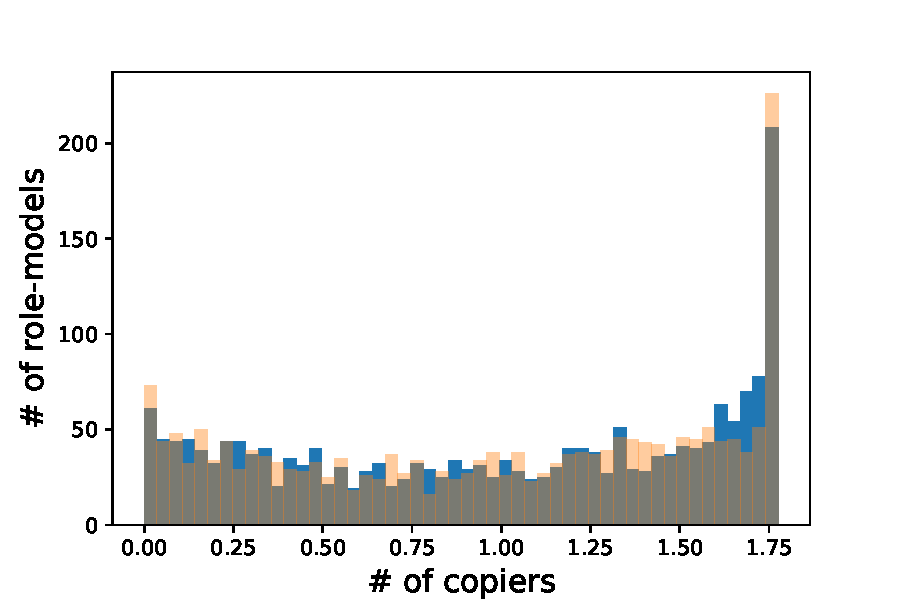
\includegraphics[width=0.7\linewidth]{../figures/final/GBD_validation.pdf}
  \caption{
  \textbf{Numerical validation of the GB approximation.}
  The approximation (orange) fits simulation results (blue) well when using 1,000 simulations for both models.
  Here, population size, $N=2,000$; bias weight, $\alpha=0.1$; idea phenotype value, $\hat{A}=1$; role-model traits $\vec{A} \sim N(0,1)$; success bias value, $\beta(A)=0.956$.}	
  \label{fig:GBD}
\end{figure}

Although basic, \Cref{fig:GBD} shows good fit of the GB approximation.
This validation is initial, and the more extensive validations we do on the Dirichlet-Multinomial approximation, because it is what we will use in our analysts.

%%%%%%%%%%%%%%%%%%%%%%%%%%%%%%%%%%%
\subsection*{Dirichlet-Multinomial distribution approximation}

\paragraph{P\'{o}lya urn model.}
This stochastic process consists of $N$ draws from an urn with an initial amount of colored balls of $M$ colors. When a ball is drawn, it is then placed back in the urn together with an additional new ball of the same color.
Let $\vec{U_i} = \{u_{i,1},u_{i,2},...,u_{i,M}\}$  where $u_{i,j}$ is the number of balls of the $j$-th color in the urn after $i$ draws.
Let $S_{i,j}=1$ when drawing a $j$-colored ball on the $i$-th draw, and $0$ otherwise. The probability that $S_{i,j}=1$ given $\vec{U_{i-1}}$ is
\begin{equation}\label{eq:polya}
\begin{split}
P(S_{i,j} = 1 \mid \vec{U_{i-1}}) = 
\frac{u_{i-1,j}}{\sum\limits_{m=1}^{M} u_{i-1,m}} = 
\frac{o_j + w_{i-1,j}}{\sum\limits_{m=1}^{M} o_m + w_{i-1,m}} = 
\frac{o_j + w_{i-1,j}}{i-1 + \sum\limits_{m=1}^{M} o_m} \;,
\end{split}
\end{equation}
where $o_j$ is the initial number of balls of the color $j$ in the urn, and $w_{i,j}$ is the cumulative number of new balls that were added to the urn after $i$ draws of the color $j$.
\\

\begin{result}[P{\'{o}}lya urn model]\label{result:polya}
The role-model choice process, $\big\{\vec{K}_i\big\}_{i=1}^N$, is equivalent to a \emph{P\'{o}lya urn model} if both trait estimation error and bias weight are uniform in the population, $e=e_j$ and $\alpha=\alpha_j$ for all $j=1,\ldots,N$.
\end{result}

\begin{proof} 
Denote $\alpha'=\frac{\alpha}{1-\alpha}$ as the bias weight ratio, and $A'_j=A_j+e$. From \cref{eq:prestige} and because $\sum_{j=1}^{N}{K_{i,j}}=i$, we have
\begin{equation}\label{eq:copier_choose}
G_{i,j} = 
\frac{\alpha'\beta(A'_j) + K_{i-1,j}}{\sum\limits_{m=1}^{N} \alpha'\beta(A'_m) + K_{i-1,m}}
 =\frac{\alpha'\beta(A'_j) + K_{i-1,j}}{i-1 + \sum\limits_{m=1}^{N}\alpha'\beta(A'_m)} \;.
\end{equation}
Substituting $M=N$, $o_j = \alpha'\beta(A'_j)$, and $w_{i,j} = K_{i,j}$ in \cref{eq:polya} gives \cref{eq:copier_choose}, thus completing the proof.
\end{proof} 

\citet[section 2]{dirichlet} prove that the proportion of different colored balls in a \emph{P\'{o}lya urn model} converges to the Dirichlet distribution as the number of draws approaches infinity, based on the \emph{Martingale Convergence Theorem} \citep{martingaleBook}.
We therefore have an approximation for the relative prestige each role-model has when evaluated by copiers. Thus, choosing the role-models for all copiers is equivalent to drawing from a Multinomial distribution where the parameters are the modified weights from a Dirichlet distribution and we have the following corollary.
\\

\begin{corollary}\label{cor:dirichlet}
The number of copiers of each role-model follows a Dirichlet-Multinomial distribution, $\vec{K_i} \sim \emph{DM}(N,\vec{G_1})$, under the conditions of \Cref{result:polya}.
\end{corollary}

\paragraph{Numerical validation.}
To validate our analytical result (\Cref{cor:dirichlet}) and test its sensitivity to the assumptions ($e_i=e$ and $\alpha_i=\alpha$ for $i=1,\ldots,N$) we compare it to results of stochastic simulations of the full model.
First, we computed an observed distribution of the number of copiers from the average empirical distribution of multiple simulations.
We then compared this observed distribution with the expected theoretical DM distribution as can be seen in \Cref{fig:DM_validation} (a). The difference in distributions was not perceived when plotting both distributions on the same figure, so we used the difference instead. The maximum difference is 0.5 role-models, which indicate a very good fit.
In addition, we tested the likelihood of the observed data to be drawn from the DM distribution, against a shuffle of the parameters vector of the DM distribution itself, as seen in \Cref{fig:DM_validation} (b). We see that the negative log likelihood of the observed data is much higher than any other shuffled version of the parameters vector, supporting our approximation more.


\begin{figure}[h]
    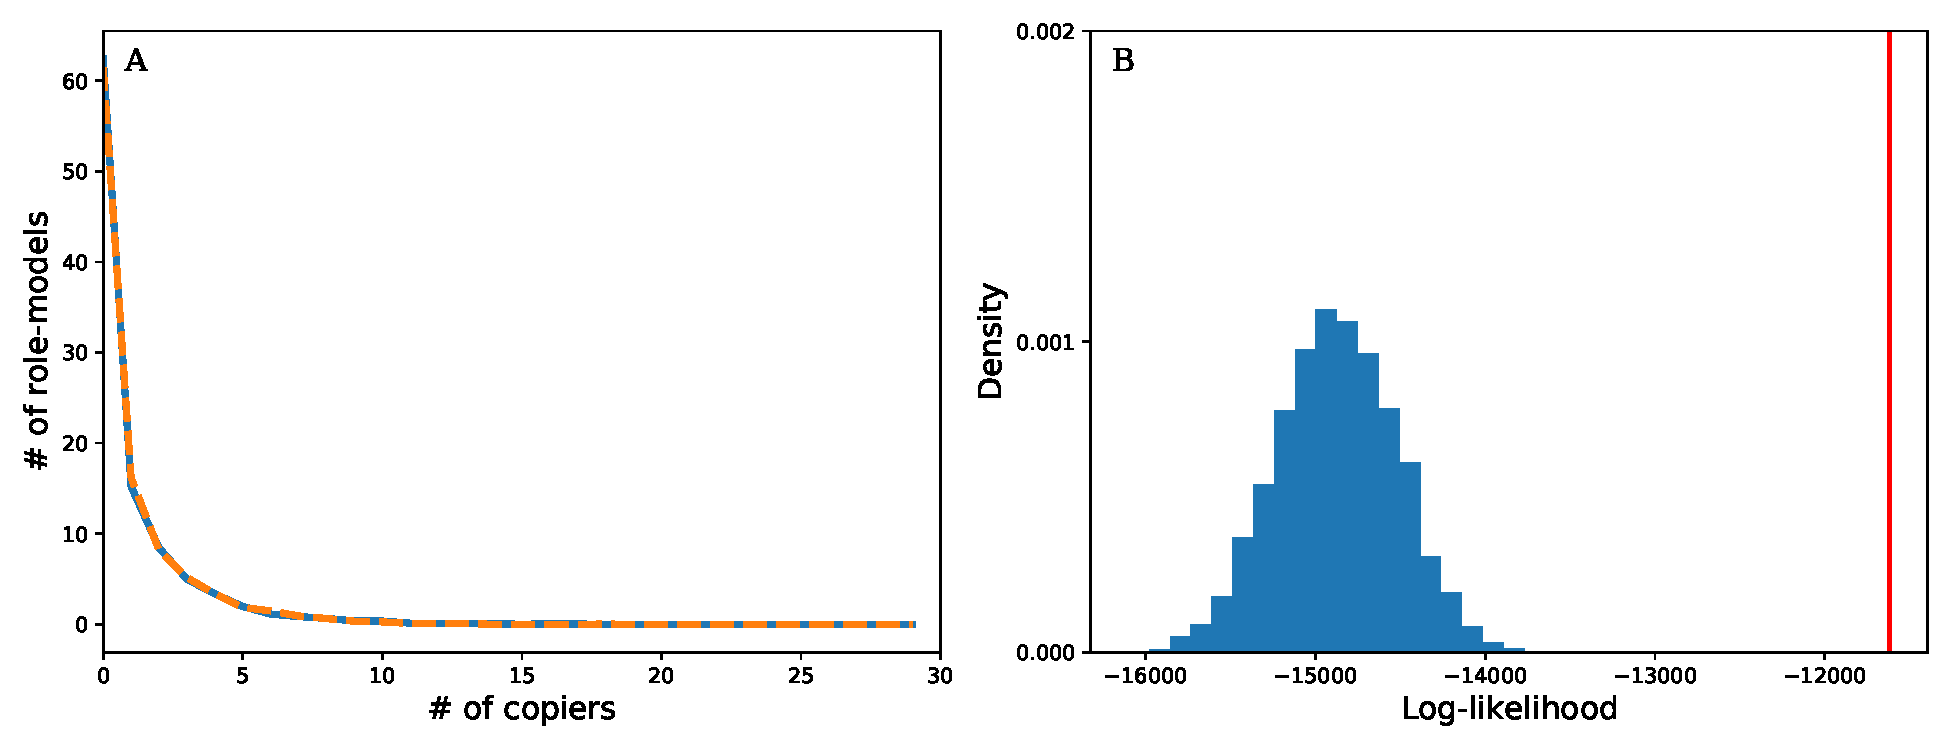
\includegraphics[width=\linewidth]{../figures/final/DM_validation.pdf}
  \caption{
  \textbf{Numerical validation of the DM approximation.}
  We performed computational "experiments" of the role-model choice process and compared them to the DM distribution. 
  \textbf{(A)} The difference between the DM distribution (orange) and the empirical distribution of the experiments (blue) is very small. 
  \textbf{(B)} The log-likelihood of the DM distribution for results of the experiments (red vertical line) is much higher compared to the log-likelihood of permutations of experiments (blue histogram).
  Here, population size, $N=100$; number of experiments, $m=100$; phenotype values, $\hat{A}=1$, $A \sim N(0,1)$; success-bias weight, $\alpha=0.5$.
  No estimation error or bias is applied, and traits are estimated and copied perfectly.}	
  \label{fig:DM_validation}
\end{figure}


Next, we examined the fixation probability and fixation time of a favored phenotype $\hat{A}$ when invading a population of phenotype $A$ and compared results from the full model and the DM approximation.
Thus, we assume the population has a single individual with phenotype $\hat{A}$ and $N-1$ individuals with phenotype $A$. 
We find that the number of simulations needed to sufficiently approximate our model with the DM approximation is roughly $1,000$ (\Cref{fig:num_sims}).
We examined the robustness of the DM approximation to relaxing the approximation assumptions.
First, we relaxed our assumption of no estimation error $e$.
Estimation error in the original model was drawn from a normal distribution, and added to the trait value before evaluation of the bias ($A_{ij} = A_j + e_i$).
When estimation error is applied, we sample $J_i$ for each copier $i$ from a normal distribution with varying scale (variance).
Even when the standard deviation is $0.1$, the fixation probability and time is similar~(\Cref{fig:hetro_error}). 
We also relaxed our assumption of a uniform bias weight $\alpha$ (i.e., $\alpha_i=\alpha$). We allowed $\alpha$ to vary in the population, drawing $\alpha_j$ for each role-model $j$ from a normal distribution such that $\alpha_j \sim N(0.5,q)$ where $q \in [10^{-7},10^{-1}]$. 
We found again that results of the DM approximation are similar to those from stochastic simulations of the full model~(\Cref{fig:hetro_alpha}).



\begin{figure}[h]
    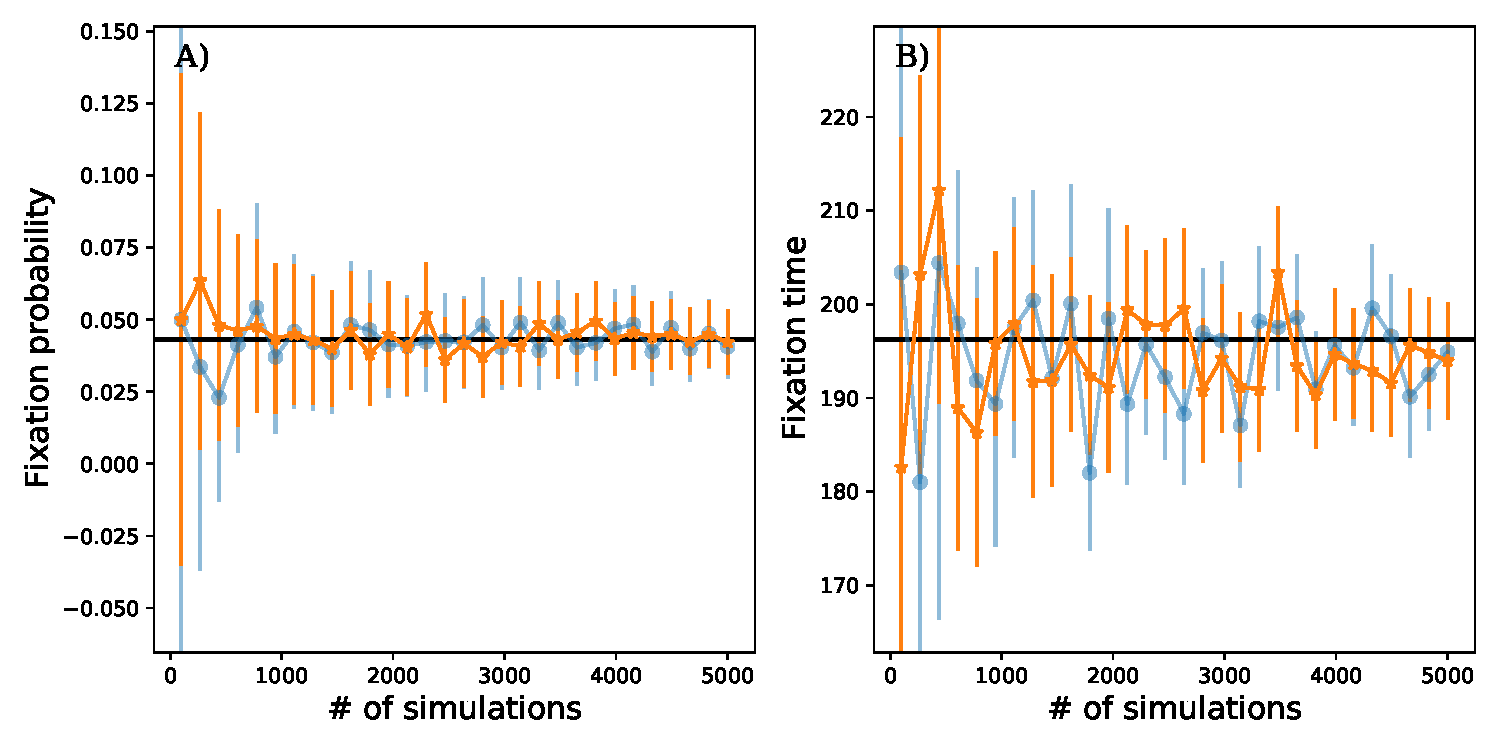
\includegraphics[width=\linewidth]{../figures/final/num_sims.pdf}
  \caption{
  \textbf{DM Approximation precision as function of number of simulations.}
  Our DM approximation (orange) agrees with stochastic simulation results (blue) when using 1,000 or more simulations.
  Both fluctuate around the analytic fixation probability approximation (black; \cref{eq:kimura_p}).
  Markers are averages across simulations, error bars are 95\% confidence intervals.
  Here, population size, $N=1000$; success-bias weight, $\alpha=0.5$; phenotype values, $\hat{A}=1$, $A=0.7$; success-bias value, $\beta(A)=0.956$.}	
  \label{fig:num_sims}
\end{figure}


\begin{figure}
    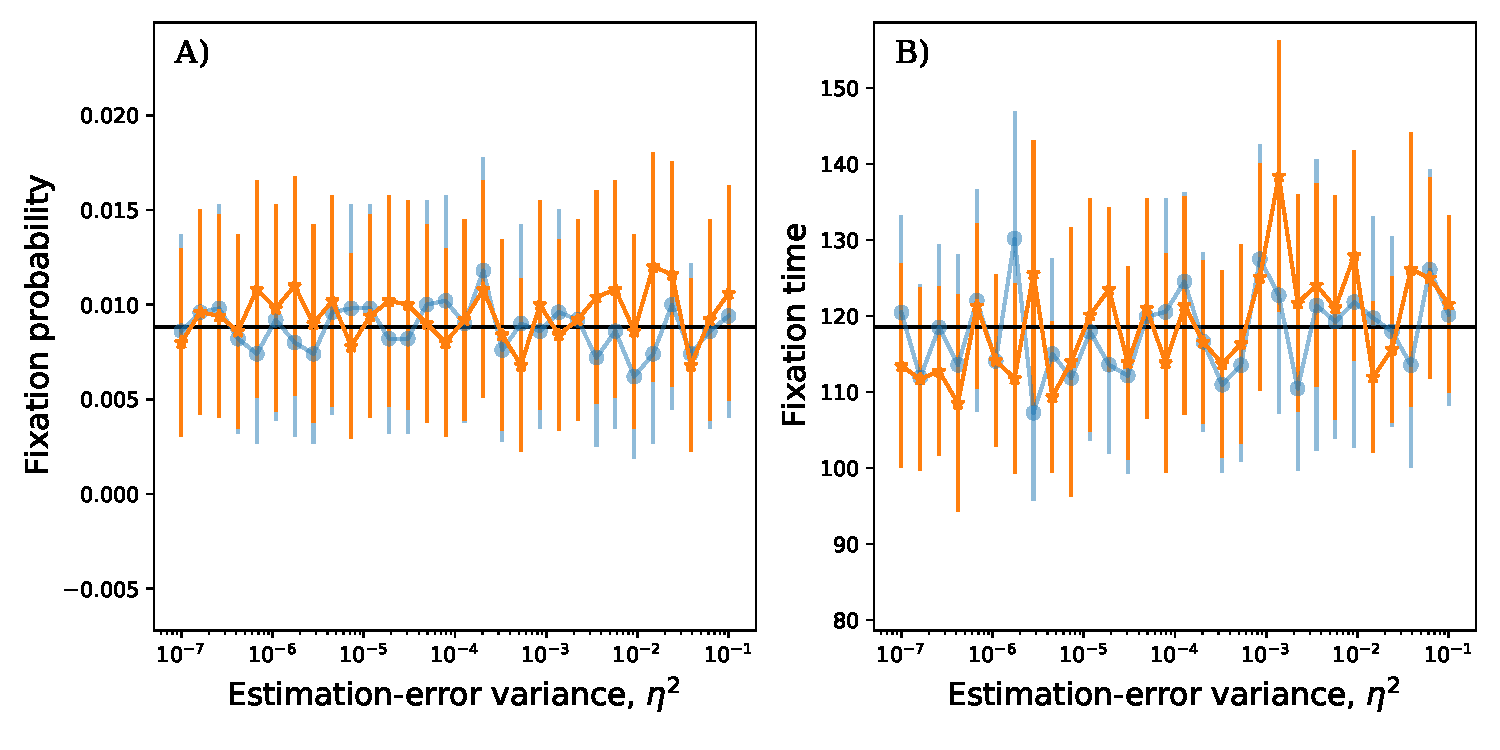
\includegraphics[width=\linewidth]{../figures/final/full_vs_dm_mutation.pdf}
  \caption{
  \textbf{Robustness of DM approximations to success estimation error.}
  Both the DM approximation (orange) and our approximation (black) agree with the stochastic simulations (blue), even with a high estimation error.
  Markers are averages across simulations, error bars are 95\% confidence intervals.
  5,000 simulations per data point; population size, $N=1000$; success-bias weight, $\alpha=0.1$; phenotype values, $\hat{A}=1$,$A=0.7$; bias strength parameter $J\sim N(1,\eta^2)$ where $\eta \in [10^{-7},10^{-1}]$.
  }	
  \label{fig:hetro_error}
\end{figure}


\begin{figure}
    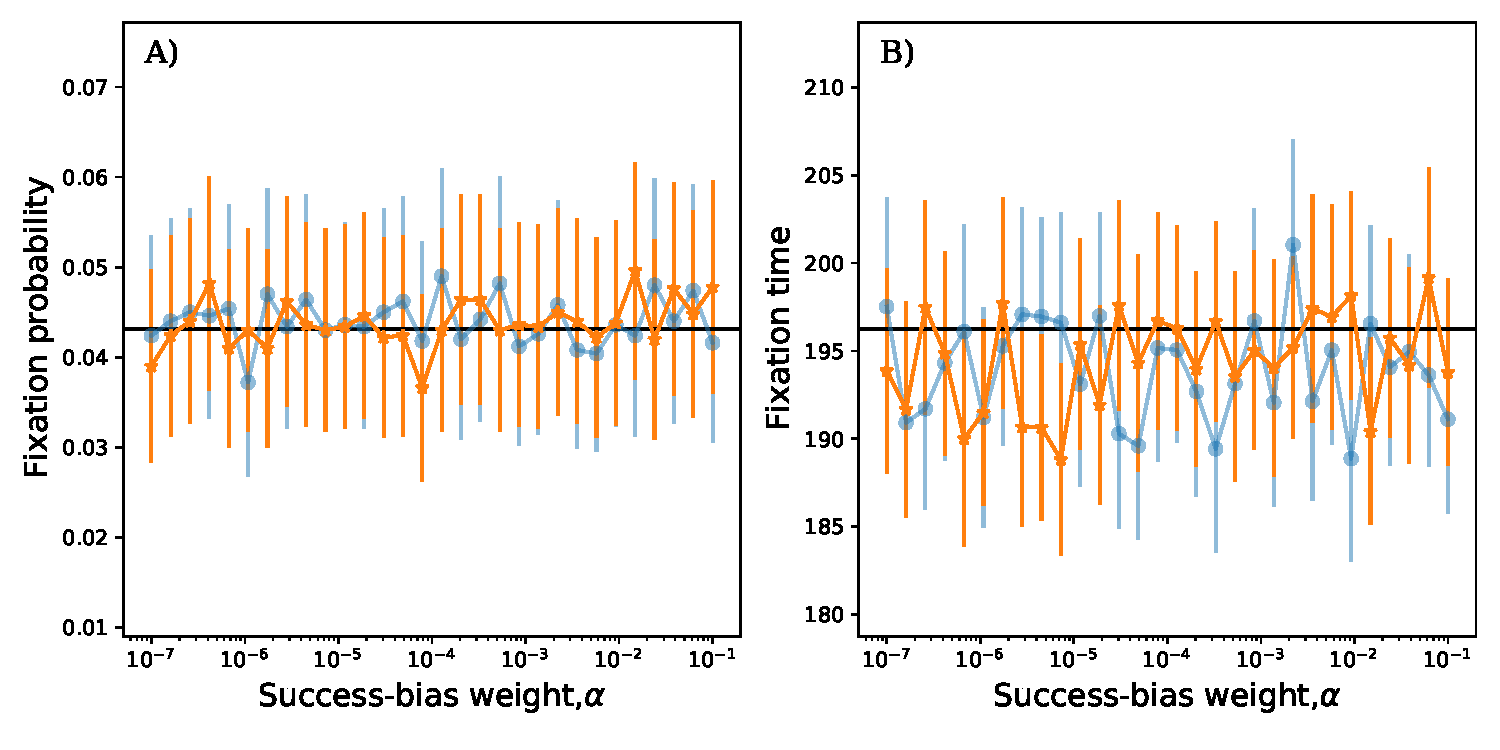
\includegraphics[width=\linewidth]{../figures/final/full_vs_dm_changing_alpha.pdf}
   \caption{\textbf{Robustness of DM approximations to variation in the bias weight $\alpha$.} 
   Both the DM approximation (orange) and Kimura's equation (black line) fit the stochastic simulations (blue) well even with a high variation in success bias weight.Markers for average across $5,000$ simulations, error bars are 95\% confidence intervals.
  Here, population size, $N=1000$; success bias weight normally distributed, $\alpha\sim N(0.5,x^2)$; phenotype values ,$\hat{A}=1$,$A=0.7$; success bias value, $\beta(A)=0.956$.}	
  \label{fig:hetro_alpha}
\end{figure}


%%%%%%%%%%%%%%%%%%%%%%%%%%%%%%%%%%%%%%%%%%%
\subsection*{Fixation probability and time}

After finding that the DM distribution is a good approximation of the (within-generation) role-model choice process, we turn our attention to the (between-generation) evolutionary dynamics.
We focus on the fixation probability and conditional fixation time (conditioned on the population reaching fixation) of a favored phenotype, using a diffusion-equation approximation approach, similar to analyses of population-genetic models \citep{kimura,kimura_average,otto_fixation}.
We are mainly interested in the effect of the bias weight, $\alpha$, which determines the relative effect of success and influence on prestige bias, given by \cref{eq:prestige}.
For simplicity, we do not include role-model estimation error in this analysis, i.e $e_i=0$ for every copier $i$.
As shown above, transmission in our model is approximately DM distributed (\Cref{cor:dirichlet} and \cref{eq:copier_choose}).

We start by finding the expectation and variance of the change in frequency from one generation to the next, which are the drift and diffusion terms of the diffusion equation.
The proof is in Appendix~\ref{sec:drift_diff_const}.
\\

\begin{result}[Drift and diffusion terms in a constant environment]
Let $x$ and $x'$ be the frequency of type $\hat{A}$ in a population with $N$ individuals in the current and next generation, and  $\beta$ is the success coefficient of phenotype $A$, $\beta = \beta(A) < \beta(\hat{A}) = 1$.
Then,
\begin{equation}
E[x'-x] \approx x(1-x)(1-\beta) \;, 
\quad
V(x'-x) \approx x(1-x)\Big(\frac{1}{\alpha N + (1-\alpha)}\Big) \;.
\end{equation} 
\end{result}


This analysis gives a surprising result relating the parameters $\alpha$ and $\beta$ to parameters of the classical Wright-Fisher model from population genetics:
the selection coefficient $s$, a measure of the effect of natural selection on the change in frequency of genotypes, and the effective population size, $N_e$, a measure of the effect of random genetic drift on the change in frequency of genotypes. 
In a diffusion-equation approximation of the classical Wright-Fisher model, the expectation and variance of the change in frequency are $E[x'-x]=x+x(1-x)s+o(s)$ and $V[x'-x]=x(1-x)/N_e$ \citep[eq.~7]{kimura}. 
Therefore, we have the following result.\\

\begin{result}[Effective selection coefficient and population size]\label{res:selection_coef}
The effective selection coefficient $s$ and effective population size $N_e$ can be written in terms of the success coefficient $\beta$ (\cref{eq:success_bias}), the bias weight $\alpha$ (\cref{eq:prestige}), and the population size $N$ as 
\begin{equation}
s=1-\beta(A), \quad N_e=\alpha N + (1-\alpha) \;.
\end{equation}
\end{result}

Note that when $N>>1$, $N_e \approx \alpha N$, resulting in a very convenient expression.\\

Using our effective selection coefficient, $1-\beta$, and effective population size, $N_e$, with the population-genetics fixation probability approximation given by \citet[eq.~8]{kimura}, we get the following result:
\begin{result}[Fixation probability]
The fixation probability is approximately
\begin{equation}\label{eq:kimura_p}
\pi(x) = \frac{1-e^{-2(1-\beta)N_e x}}{1-e^{-2(1-\beta)N_e}}
\end{equation}
where $x$ is the initial frequency of the favored phenotype $\hat{A}$.
\end{result}

Similarly, we can use $1-\beta$ and $N_e$ in the population-genetics fixation time approximation given by \citet[eq.~17]{kimura_average}.\\

% TODO SAAR check these equations vs what you have in the source code
\begin{result}[Fixation time] The fixation time (conditioned on fixation) from an initial frequency $x$ is approximately
\begin{equation} \label{eq:kimura_t}
T(x) = J_1(x) + \frac{1-\pi(x)}{\pi(x)}\cdot J_2(x),
\end{equation}
where $N_e=\alpha N + (1-\alpha)$, $S=N_e(1-\beta)$, and
\begin{equation}
\begin{aligned}
J_1(x) &= \frac{2}{(1-\beta)(1-e^{-2S})}\int_x^1 \frac{(e^{2S\xi}-1)(e^{-2S\xi}-e^{-2S})}{\xi(1-\xi)}d\xi \;, \\
J_2 (x) &= \frac{2}{(1-\beta)(1-e^{-2S})}\int_0^x \frac{(e^{2S\xi}-1)(1-e^{-2S\xi})}{\xi(1-\xi)}d\xi \;.
\end{aligned}
\end{equation}
\end{result}
Note that these integrals cannot be solved in closed form, so we can only estimate them numerically.

\paragraph{Numerical validation.}
We compare our approximations (\cref{eq:kimura_p,eq:kimura_t}) with results of simulations of our dichotomous model using various $\alpha$ and $\beta$ values, as well as simulations of the Wright-Fisher model, using the effective selection coefficient, $1-\beta$, and effective population size, $N_e=\alpha N + (1-\alpha)$. 
We find see that the two models have similar dynamics, and both are well approximated our approximations (\Cref{fig:var_alpha}).


\begin{figure}[h]
    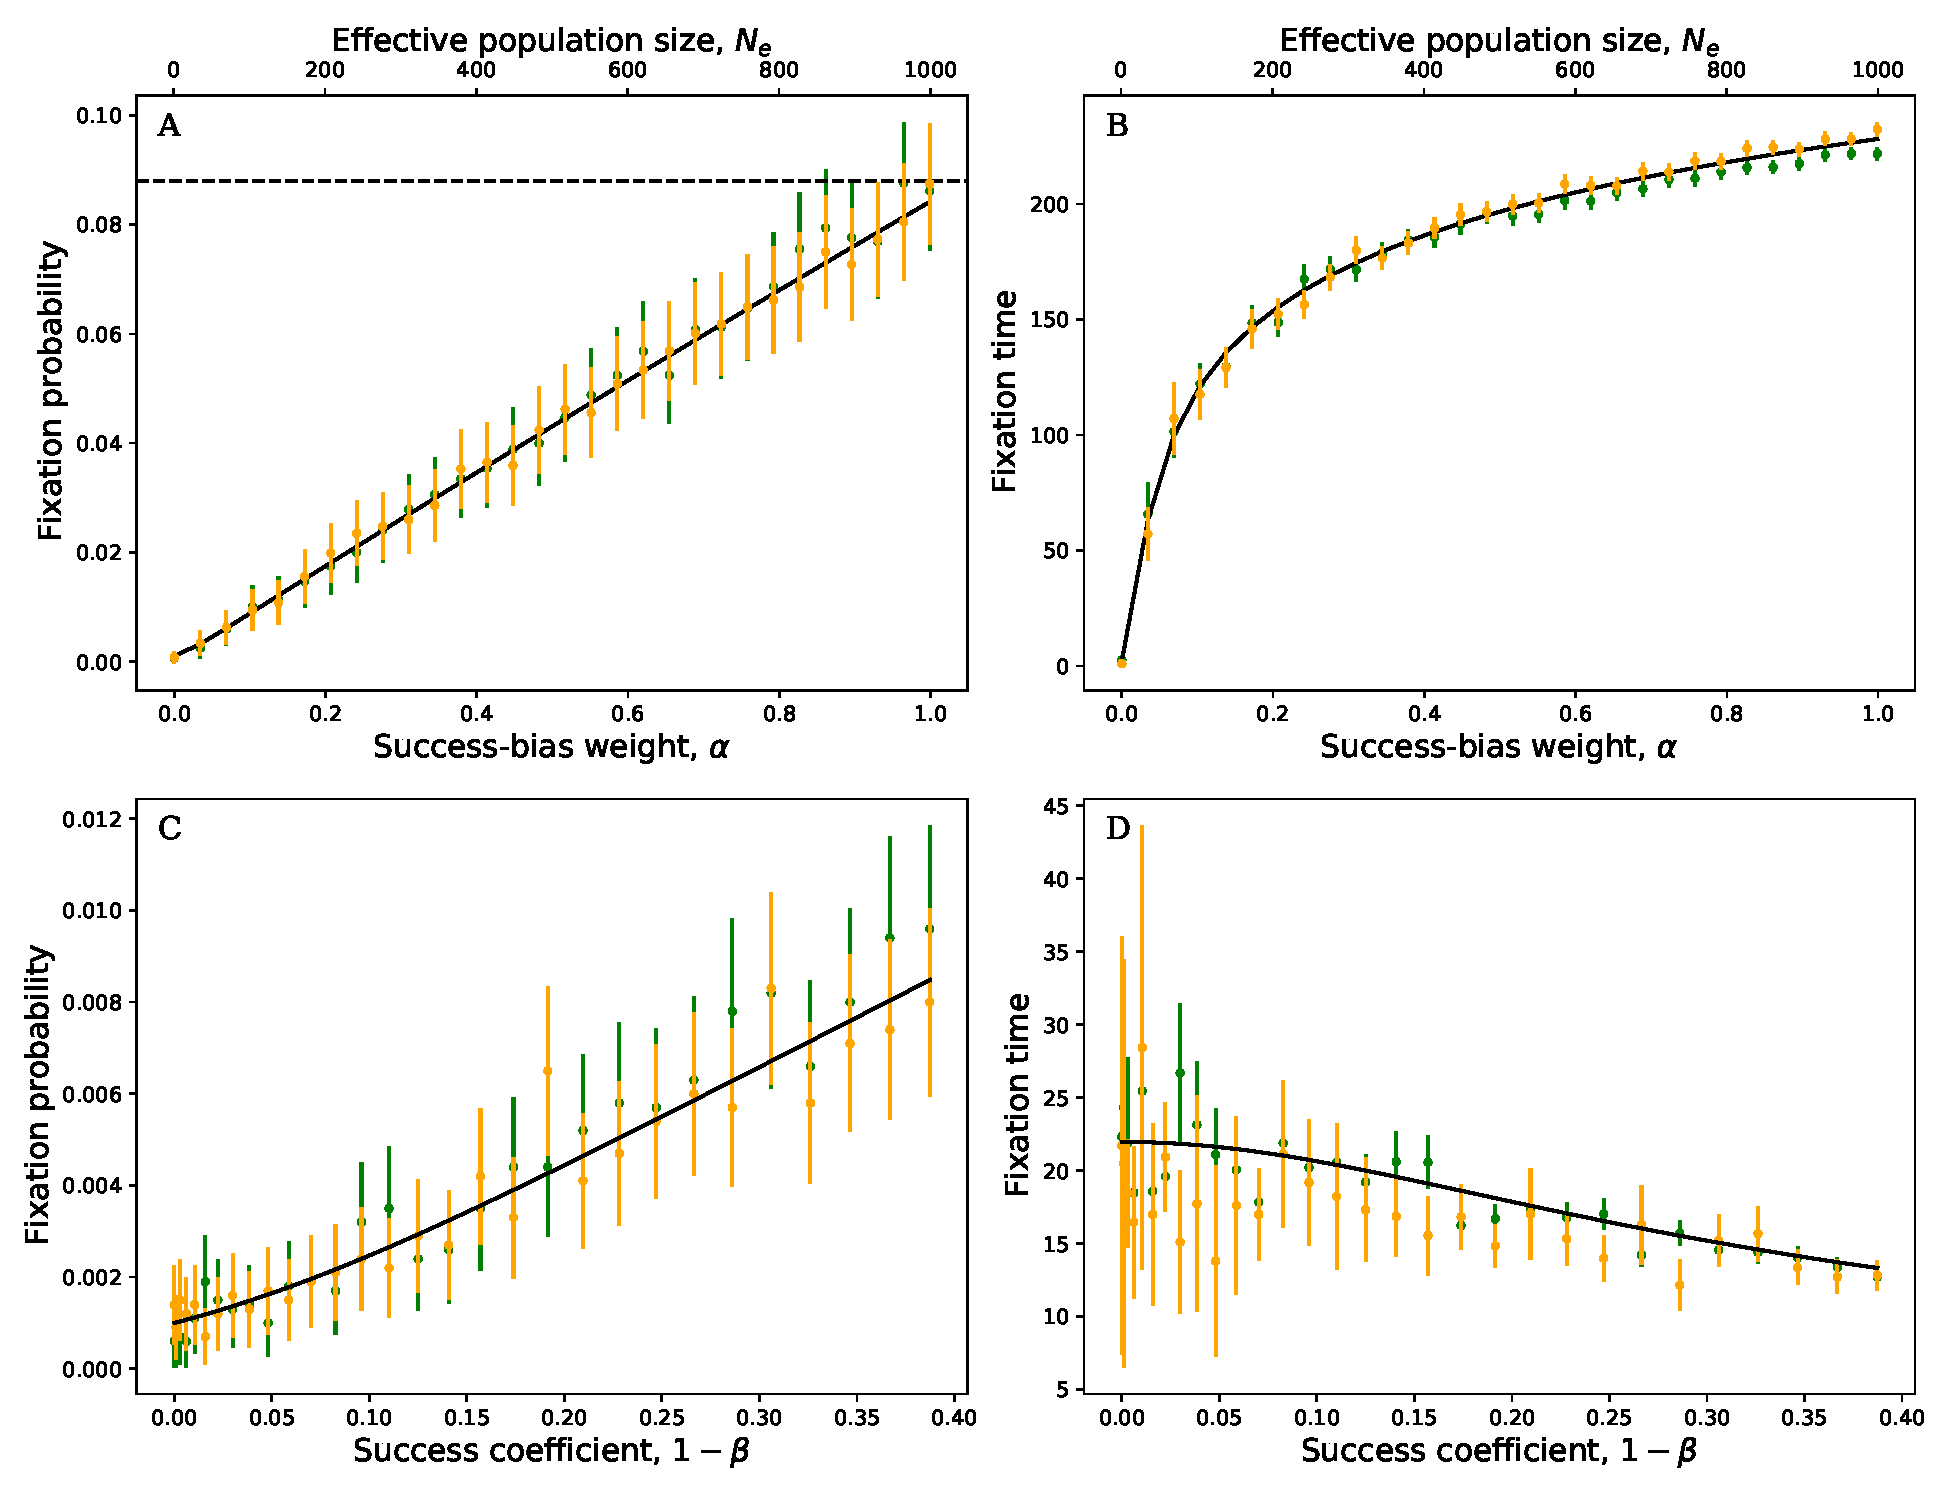
\includegraphics[width=\linewidth]{../figures/final/kimura_var.pdf}
  \caption{\textbf{Fixation probability and time in a constant environment.}
  Fixation probability and time (in generations) as a function of the success-bias weight $\alpha$ (bottom x-axis), or effective population size $N_e$ (top x-axis) in the top row, and as a function of the success coefficient, $1-\beta$, on the bottom row.
  The approximation (black; \cref{eq:kimura_p}) agrees with both DM simulations (green) and Wright-Fisher simulation (orange).
  Fixation probability (A) is bounded by $2(1-\beta)$ (blue).
  Markers are averages of $10,000$ simulations, error bars show 95\% confidence intervals for panels A and B and 75\% for panels C and D.
   Here, Population size, $N=1,000$; phenotype values, $\hat{A}=1$, $A=0.7$ (A and B), $A = a \cdot \hat{A}$ with $0.01 \le a \le 0.99$ (panels C and D); success coefficient, $1-\beta=s=0.044$ (A and B); success-bias weight, $\alpha=0.01$ (panels C and D).}
  \label{fig:var_alpha}
\end{figure}


\paragraph*{Changing environment}. After finding a good approximation in constant environment, where the favorable trait is always $\hat{A}$, we proceeded to find an approximation for a changing environment. 
Following \citet{changeEnv}, we denote $k$ as the number of generations in which the invading phenotype is favored by success bias, and $l$ as the number of generations in which the resident phenotype is favored by success bias.
We then proceed to find expressions for the expectation and variance of the change in frequency between $n=k+l$ generations. 
The proof is in Appendix~\ref{sec:drift_diff_chang}.
\\

\begin{result} [Drift and diffusion terms in a changing environment]\label{res:ch_expected}
Let $x$ be the initial frequency of the invading phenotype and $X_t$ is the number of individuals with the phenotype after $n$ generation.
Then,
\begin{equation}\label{eq:ch_expected_and_var}
E[X_n/N - x] \simeq x(1-x) S_n / N_e \;, 
\quad
\text{and}
\quad
V(X_n/N-x) \simeq  n x(1-x) / N_e \;,
\end{equation}
where $S_n=\sum\limits_{t=1}^{n} N (1-\beta_t)$.
\end{result}

Note that here, we have the average selection coefficient during a cycle of $n$ generations as the selection coefficient \cref{eq:kimura_p}.
Using the drift and diffusion terms and following \citet{changeEnv}, we can approximate the fixation probability in a changing environment using
\begin{equation}\label{eq:ch_env}
\tilde\pi(x) = \frac{1-e^{-2 \frac{S_n}{n} N_e x}}{1-e^{-2 \frac{S_n}{n} N_e}} \;.
\end{equation}

\paragraph{Numerical validation.}
% TODO SAAR edit this section
Comparing our approximation (\cref{eq:ch_env}) to simulations, we find that the approximation fits simulation results well for variable bias weights, $\alpha$, which corresponds to the effective population size (\Cref{fig:ch_env_alpha_beta}A).

However, the approximation is more sensitive to the value of the success bias coefficient $\beta$ (\Cref{fig:ch_env_alpha_beta}B).
We suspect that when $\beta$ is too small, there will not be many cycles in the simulations, because either the population reaches a high frequency of the fitter phenotype after just a few cycles, or the fitter phenotype becomes extinct very quickly. 
For such $\beta$ values (below 0.65), the fixation probability exceeds even the constant environment approximation (which is the upper limit). We note that the diffusion-equation approximation assumes weak selection, or in our case, weak success bias.

We found that for a large $k/l$ ratio (with a constant cycle length, $n=k+l=100$), the changing environment approximation (\cref{eq:ch_env}) converges to the constant environment approximation (\cref{eq:kimura_p}), see \Cref{fig:ch_env_alpha_beta}C and \Cref{fig:ch_env_alpha_beta}D.

The approximation follows the trend of the simulation results for all $\alpha$ values.
When increasing the success coefficient to more than 0.15, the simulation results were located above the changing environment approximation, and below the constant environment approximation. We believe the reason is the structure of the cycle.
Our proof and approximation in the changing environment are for a large amount of cycles, and when the success coefficient is too high, there might be very few cycles. Either the ideal trait is copied by enough copiers so that the influence is sufficient to negate the success bias when the cycle changes (and the trait favored by the bias becomes the disfavored), or the opposite happens, and the ideal trait gets extinct before there were enough copiers that copied it.
We then tried to change the ratio between the number of cycles where $\hat{A}$ is favored and disfavored. We showed that the approximation fits well regardless of the ratio, but when the ratio of favored generations to disfavored ones is very high, it is very similar to a constant environment model.



\begin{figure}[H]
    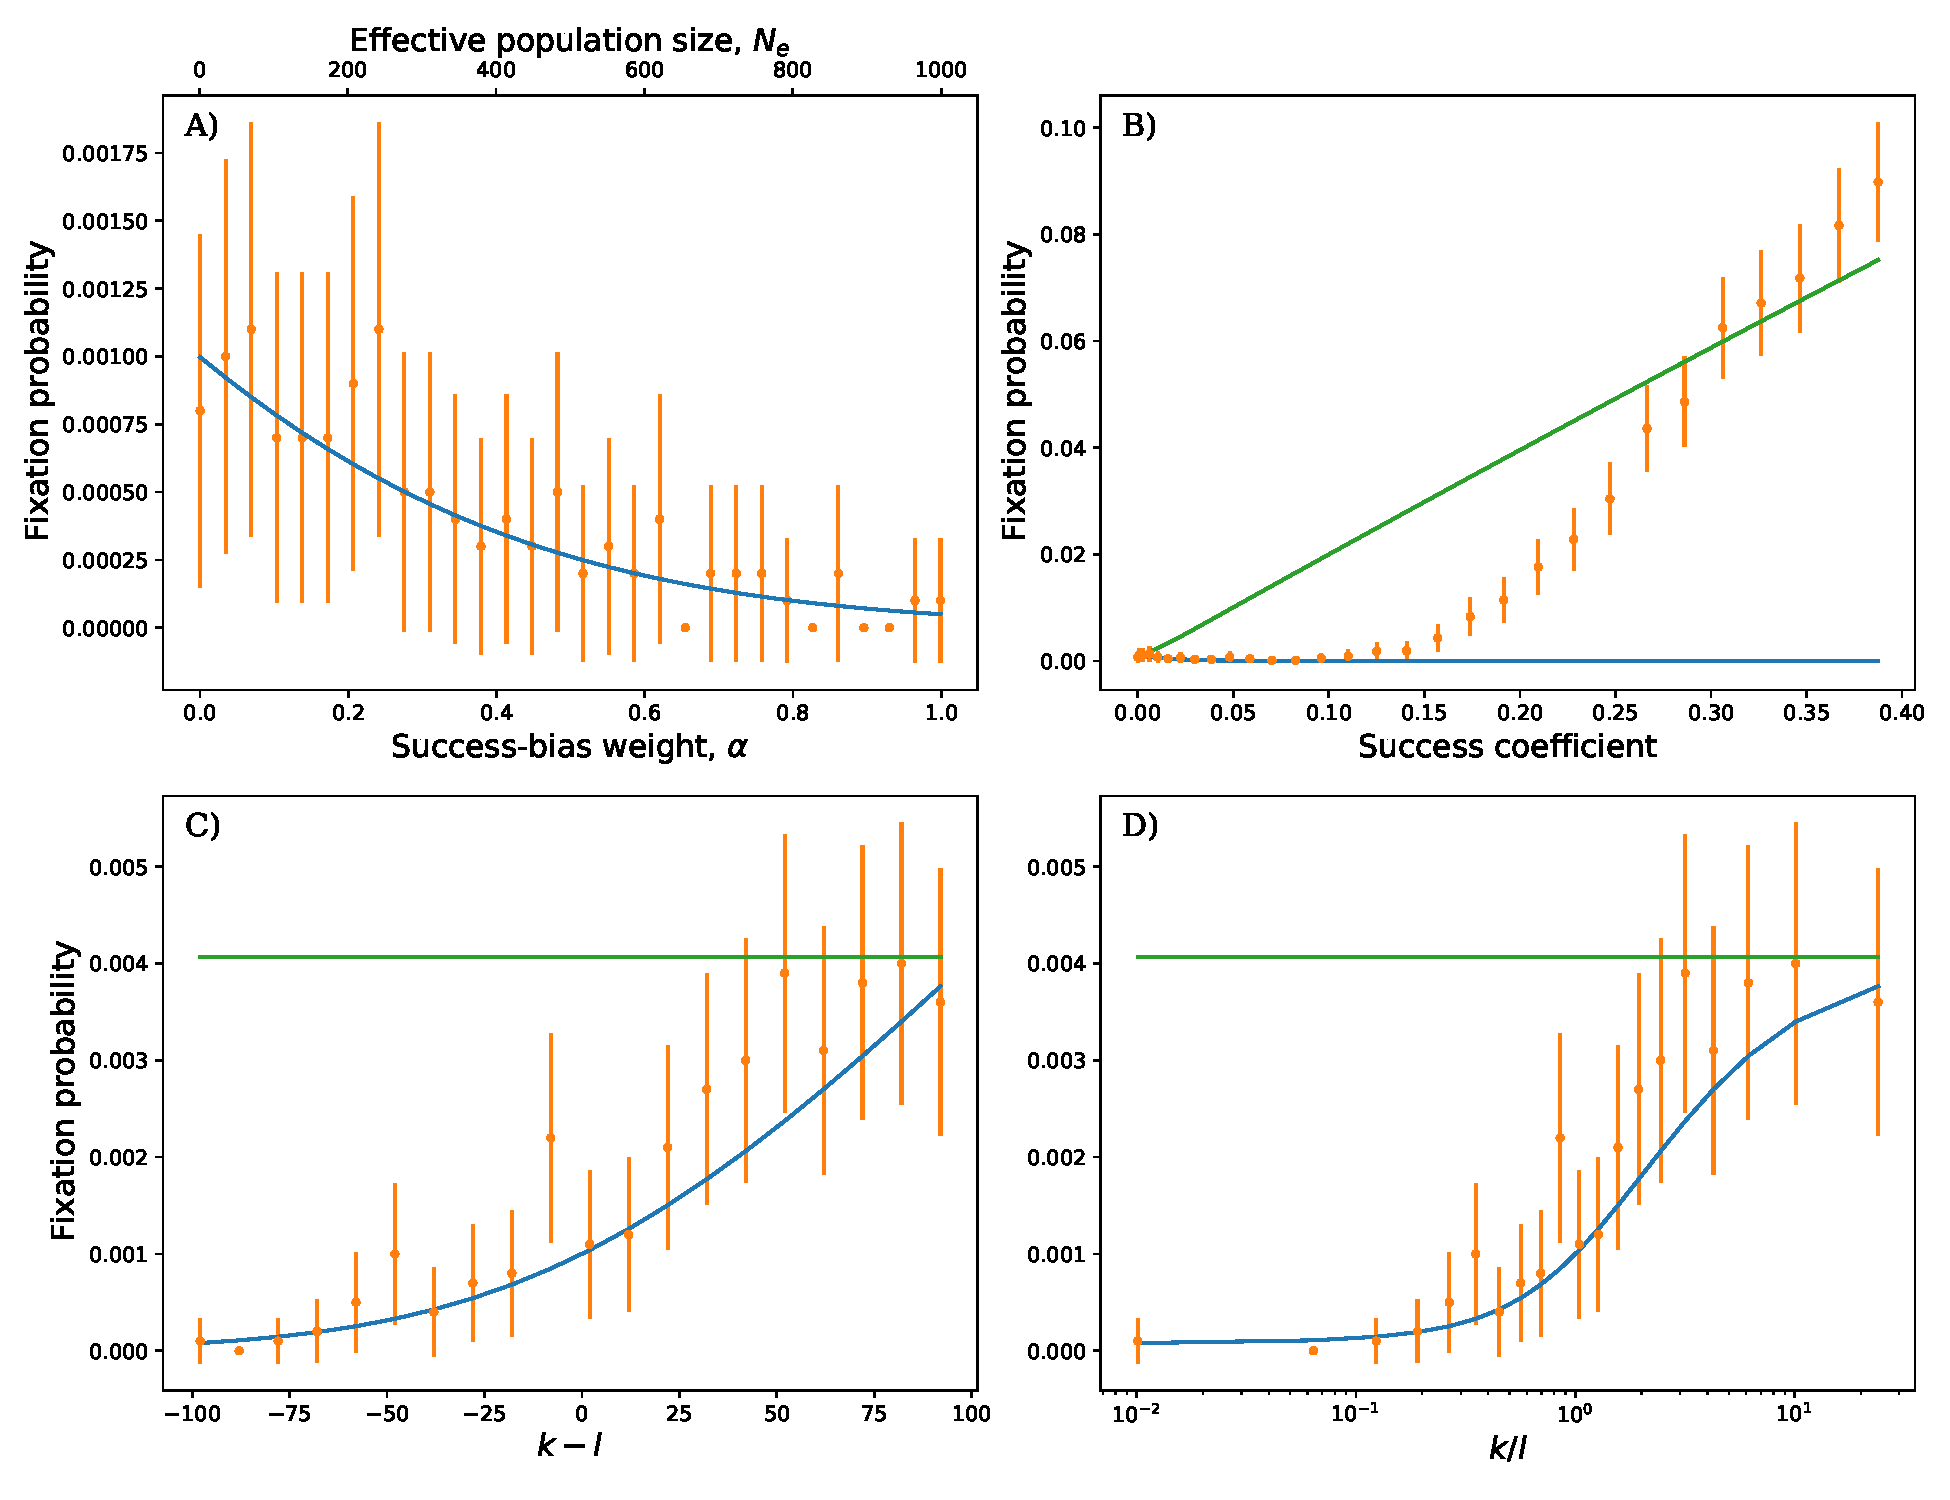
\includegraphics[width=\linewidth]{../figures/final/ch_env.pdf}
  \caption{\textbf{Fixation probability in a changing environment.}
\textbf{(A)} Fixation probability decreases with the the success-bias weight (bottom x-axis) and effective population size (top x-axis). The approximation (blue; \cref{eq:ch_env}) agrees with simulation results (orange). 
\textbf{(B)} Fixation probability increases with the success coefficient, $\beta$.
When success bias is large ($1-\beta > 0.1$),  
simulation results (orange) are underestimated by the changing environment approximation (blue; \cref{eq:ch_env}). With even larger success bias ($1-\beta > 0.35$), even the constant environment approximation (green; \cref{eq:kimura_p}) slightly underestimates simulation results, likely because the diffusion equation approximation assumes weak "selection" .
(\textbf{C,D}) The approximation (blue) is robust to changes in environmental cycle length, as it agrees with simulations (orange) for different sizes of the changing environment cycle, where $k$ and $l$ are the number of generations each trait value is under success bias. 
When $k>l$, the approximation and the simulations are both very close to the constant environment approximation (green), because the more generations the rare phenotype is favored, the more similar it is to the constant environment model, where it is always favored by the success bias.
Markers show average of $10,000$ simulations, error bars show 75\% (A, C, and D) and 95\% (B) confidence intervals.
  Here, population size, $N=1,000$; phenotype values, $\hat{A}=1$, $A=0.9$ (A and B), $A=0.8$ (C and D); In (A), the success coefficient is: $1-\beta=s=0.005$; In (B, C, and D) the success-bias weight is $\alpha=0.1$.}
  \label{fig:ch_env_alpha_beta}
\end{figure}


%%%%%%%%%%%%%%%%%%%%%%%%%%%%%%%%%%%%%%%%%%%%%%%%%%%%%%
\subsection*{Adaptive success-bias weight}

We ran simulations of the role-model choice process during a single generation in which every copier evaluates its own optimal success-bias weight, $\alpha^*$, which minimizes the expected squared error between the estimated and the ideal trait values,
\begin{equation}
\alpha^* = \emph{argmin} \sum_{j=1}^N\frac{\alpha A_j + (1-\alpha) K_j}{\sum_{l=1}^N\alpha A_l + (1-\alpha) K_l} (\hat{A}-A_j)^2 \;,
\end{equation}
where $A_j$ is the trait of role-model $j$ and $K_j$ the number of copiers that already chose role-model $j$.

We find that when copiers adapt their success-bias weight, it decreases with the number of copiers that have already chosen a role-model~(\Cref{fig:influence_advantage}).
Moreover, their estimation error is much lower compared to a constant success-bias weight, which gives roughly the same high estimation error to all copiers (compare \Cref{fig:influence_advantage}B and C): in this example, the adaptive weight estimation error converges to $0.046$, whereas a constant weight gives values $>0.74$.


\begin{figure}[h]
    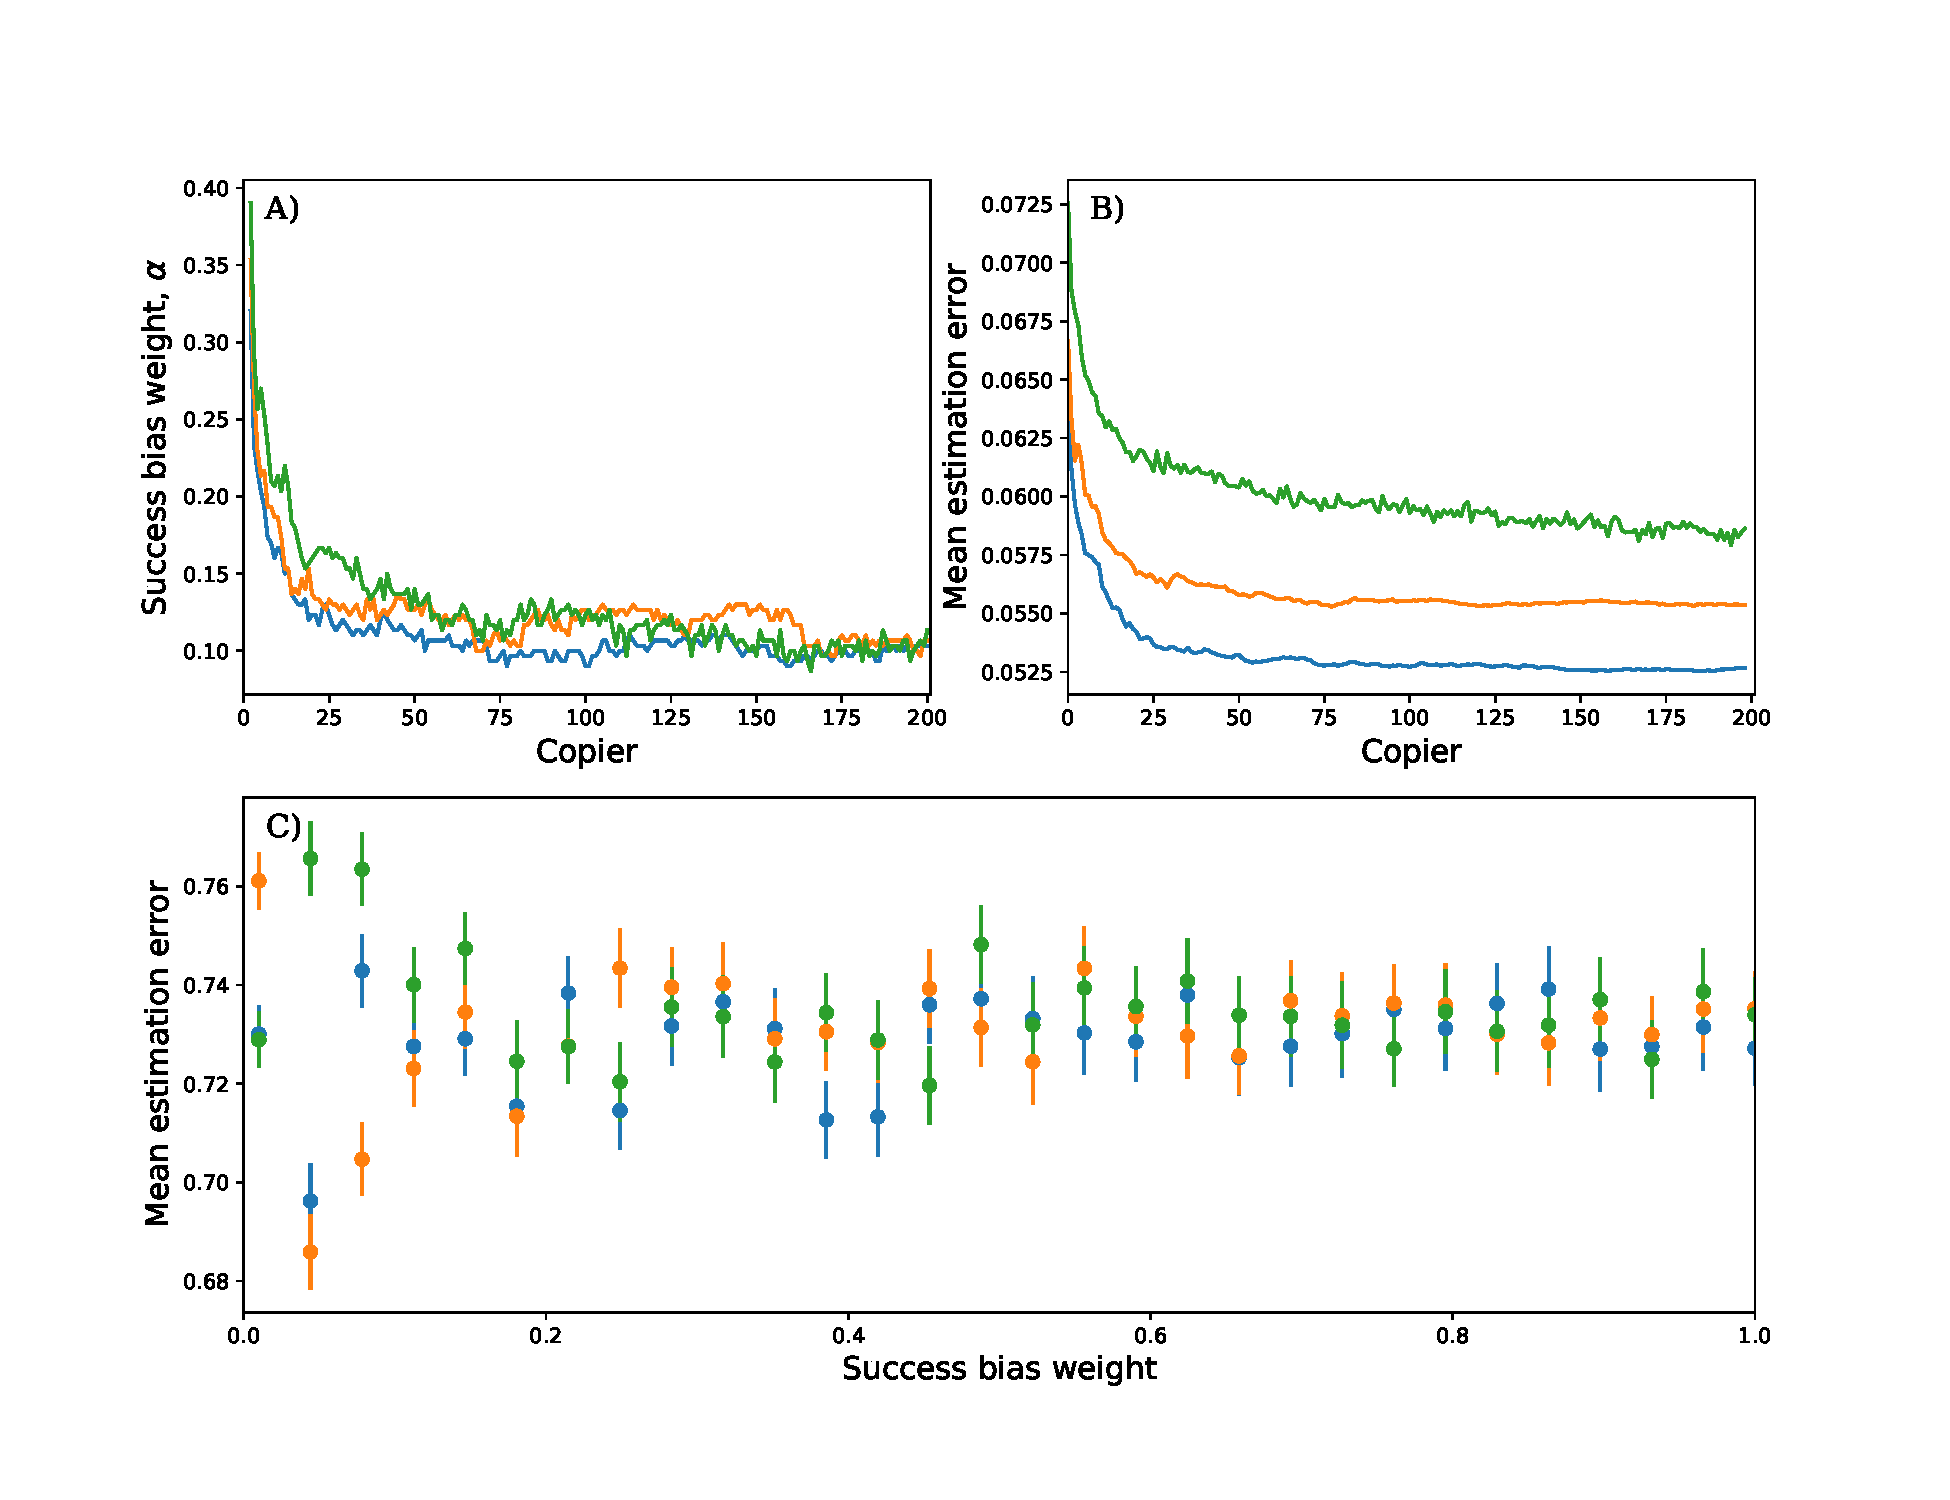
\includegraphics[width=\linewidth]{../figures/final/choose_bias.pdf}
  \caption{
  \textbf{Advantage of an adaptive success-bias weight.}
  Both success-bias weight $\alpha$ (\textbf{A}) and estimation error (\textbf{B}) decrease during the role-model choosing process, demonstrating that influence becomes more favored as more copiers have made their choice.
However, when $\alpha$ is homogeneous (\textbf{C}), the mean estimation error doesn't decrease, regardless of $\alpha$ or $\eta$.
The mean estimation error in the homogeneous $\alpha$ model is larger by a factor of $10$ than the adaptive $\alpha$ model.
Here, population size $N=200$; estimation error is normally distributed $e \sim N(0,\eta^2)$ with standard deviation $\eta=$0.0001 (blue), 0.001 (orange), 0.01 (green), plots are average of $300$ simulations.}	
  \label{fig:influence_advantage}
\end{figure}



%%%%%%%%%%%%%%%%%%%%%%%%%%%%%%%%%%%%%%%%%%%%%%%%%%%%%%
% TODO Edit to follow our latest definition of prestige etc in the introduction
\section*{Discussion}
During cultural transmission, cultural traits such as attitudes, values, beliefs, and behavioral patterns are transmitted between individuals, for example via copying and social learning.
Some cultural traits or cultural role-models may be copied more often due to transmission biases. 
A common bias is success bias, in which copiers are more likely to copy a successful role-model. Many models assume that success can be accurately estimated.
However, it has been suggested that because it is hard to estimate success, a more common bias is \emph{prestige bias}---a bias towards role-models perceived to be successful in other traits \citep{fijian_social_bias}. This perceived success can be by a manifestation of another trait, i.e indirect success, which we refer to as success in this research. Prestige can also be identified as the influence an individual has on others.

Inspired by a model by \citet{evolutionBook}, we developed a cultural-evolution model with prestige bias that includes both indirect success and influence biases, where the latter is a bias towards role-models with many copiers. This is accomplished by a role-model choice process: each copier, in its turn, chooses a role-model, and that choice is affected both by the estimated success of each potential role-model and the number of copiers that already chose each role-mode (eq.~\ref{eq:prestige}). 

This resulted in a model with two "nested" stochastic processes: the role-model choice process within each generation, and the cultural-evolutionary process between generations. To simplify the mathematical and computational analysis, we developed analytic approximations for the role-model choice process using the the {\em generalized binomial distribution} (GBD, \Cref{res:GBD}) and the {\em Dirichlet-Multinomial distribution} (DM, \Cref{cor:dirichlet}).
The latter is especially useful, as it approximates the entire role-model choice process and only requires us to assume that the relative effect of success and influence is a characteristic of the role-model, rather than the copier.

Analyzing the model with the DM distribution, we found approximations for the fixation probability and fixation time of a cultural trait under biased transmission in a constant environment.
Our approximations are similar to Kimura's evolutionary-genetic approximations, such that (i) the difference between the resident and invading cultural trait values, $1-\beta(A)$, is equivalent to the selection coefficient in favor of a beneficial allele, $s$, and (ii) increasing the relative weight of influence versus success bias, $\alpha$, decreases the effective population size, $N_e$~(\Cref{fig:var_alpha}).

We also analyzed a cyclic changing environment in which the identity of the success-biased trait switches after a fixed amount of generations~(\Cref{fig:ch_env_alpha_beta}).
We find that, similarly to the constant environment approximation, a change in the success-bias weight $\alpha$ has no negative effects on the goodness-of-fit of the approximation to simulation results.
We also showed that this approximation is more sensitive to changes in the success coefficient $\beta$ than the constant environment approximation, and a lower value is required to have a good fit. The ratio between the number of generation in which the rare phenotype is under positive transmission bias and the number of generations in which it is under negative bias does not affect the goodness-of-fit of the approximation. 

We also examined a scenario in which copiers can adapt their success-weight bias, $\alpha$, to minimize their copying error, i.e., copy trait values closer to the optimal value.
We found that as the role-model choice process proceeds (that is, more copiers make their choices), both the success-bias weight (adapted by copiers) and the estimation error decrease. 
The latter is significantly lower compared to a population using a constant, fixed success-bias weight, regardless of the value of the constant weight (\Cref{fig:influence_advantage}).
This suggests that the later a copier makes its choice, the more it should rely on choices of previous copiers, and the less it should rely on its own estimation.
The rationale, then, is that the more information a copier has, e.g. by using others as information sources, the more informative and effective his choice can be.

\paragraph{Prestige in the literature.}

According to \citet{animal_leadership}, there are two main approaches to group decision making in nature: leadership and consensus.
Leaders would usually be high-ranking members of the group: elders, individuals with many kin relations, or individuals possessing other dominant traits.
\citet{animal_leadership} describe benefits for the closest associates of a dominant baboon, such as protection from predators. 
In some species, like the females of \emph{Eulemur fulvus rufus} (Red lemur), leaders may arise due to nutritional needs, and not due to possessing superior traits \citep{lemurs}. 
In humans, leadership also has its costs and benefits. Leaders can make decisions that would most benefit them and their closest followers, while still maintaining group cohesion. 
However, wrong decision making that harms the group could result in negative effects for the leader. 
In modern society, many humans strive for prestigious positions, as they may reap rewards greater than the risk and costs to achieve them, or due to individual personality and pressure or education from the family. 

\citet{prestige_evolution} suggested that there are two types of leadership: prestige-based and dominance-based leadership.
In the latter, social status is acquired through aggression, intimidation and violence. It is also more common than prestige in non-human animals.
Their definition of prestige seems to overlap with ours. They suggest prestige is composed of estimation in the eyes of other people (similar to our success bias) and commanding position in people's minds, i.e, the number of followers other people think one has, which they define as \emph{influence}, similar to our influence bias.
\citet{prestige_evolution} show that prestige can evolve via natural selection as an efficient process to extract reproductive benefit from the flow of socially transmitted information. They back up their claims by creating testable predictions and using evidence from the literature and experiments of social sciences.
Simply put, prestige can naturally evolve when social learning already exists to save costs of individual learning. 

Furthermore, according to \citet{no_replication}, the process of cultural evolution doesn't require accurate replication of cultural traits, addressed as "representation" in their paper.
They base their assumption on three claims: mental representations are non-discrete, cultural transmission is highly inaccurate, and mental representations are not replicated, but rather are `reconstructed' through an inferential process that is strongly affected by cognitive `attractors.' They describe three different models to support their points.
We see a high similarity between their model and ours. Like them, we treat the cultural trait as non-discrete (in the main model, before simplifying it to facilitate analysis). We also assume error in estimation, such that copiers do not precisely replicate their role-models, but rather reconstruct them to create a potentially different trait, which is their representation of the role-model's trait. In addition, the inferential process that they describe as strongly affected by cognitive attractors may include our definition of influence bias.

\paragraph{Empirical evidence of prestige bias}
\citet{prestige_cultural_learning} report the first direct tests in children that suggest the existence of prestige bias, defined as the tendency to learn from individuals to whom others have preferentially attended, learned, or deferred.
Their definition of prestige is similar to our influence bias. They showed that the odds of 3-4 years-old children learning from an adult role-model to whom bystanders had previously preferentially attended for 10 seconds were more than twice those of their learning from a role-models whom bystanders ignored.
They also note that prestige effects are domain sensitive: they found that prestigious role-models were attended more when demonstrating artifact use, whereas role-models presenting food preferences had less attendants, suggesting that the domain itself (artifact use vs. food preference) can affect the attendance, and hence the prestige of the role-model.
This lead \citet{prestige_cultural_learning} to suggest that when the trait is costly to learn individually, prestige will have a stronger bias.
It would be interesting to include costs in our model to try and observe these effects and dynamics in a large population.

According to \citet{fijian_social_bias}, evolutionary theorists propose that natural selection has favored the emergence of psychological biases for learning from those individuals most likely to possess adaptive information. 
Thus, they studied Fijian villages to examine if and how such biases emerge in a small-scale society.
They found that Fijian villagers are more likely to learn from role-models perceived as more successful/knowledgeable, both within and across domains.
Their research thus suggests that copying from those perceived as successful, rather than actually are successful, is a common phenomena. 
They show that the social networks representing copier--role-model relationships are centralized, suggesting that it is consistent with the prediction that people substantially share notions about who is a good cultural model, but that individuals' role-model selections are influenced by multiple factors.

We can also find prestige bias in more modern domains such as western medicine.
\citet{medical_prestige} examined literature from 1950 to 2005 on the effects of prestige on medicinal practices. They found that active, specialized, biomedical, and high-technological types of medicine on organs in the upper part of the bodies of young and middle-aged people were accorded high levels of prestige, whereas medicine and practices with opposite characteristics had low levels of prestige. 
For example, they found that surgery counts as the most prestigious specialty, while psychiatry is the less prestigious.
In addition, doctors tend to rank practices that require more time to master as more prestigious, while other procedures that are considered easier to master are less prestigious. 
This means that there may be very important practices that are neglected due to prestige bias.
They concluded that such differences in prestige may bear consequences for actual priority setting in healthcare systems.

Prestige bias can help to cheaply estimate and acquire knowledge, which may facilitate survival and reproduction. However, it is not always the case, and there could be negative repercussions to this bias, such as invasion of maladaptive traits.
\citet{best_of_k} mention that social learning not only takes the form of random copying of other individuals, but also involves learners' choice of what to learn and from whom to learn. They suggest a best-of-k model where an individual samples~$k$ role-models and chooses the one he deems most "successful". They mentioned that a previous mathematical analysis has shown that it may sometimes result in maladaptive cultural evolution when the payoffs associated with cultural variants vary stochastically. In such a case, learners may be selectively disfavored and in the long run replaced by unbiased learners, who simply copy someone chosen at random. They developed new mathematical models that are simpler and mathematically tractable. They found that best-of-k learning, unlike unbiased learning, can facilitate the invasion of an on average inferior variant that sometimes gives a very high payoff. Our model, which includes influence bias, is consistent with this claim. When a maladaptive trait is "piggybacking" a role-model with high influence, this trait could spread in the population.
In addition, they show that best-of-k learning can be stable against invasion by unbiased learning if social learning is sometimes combined with individual learning. 
Our model only includes social learning, and not individual learning, but it could be interesting to combine it with individual learning and see how it affects the dynamics.

Prestige bias can also accelerate reversal of harmful traditions such as child marriage and domestic violence. 
\citet{harmful_traditions} suggest a \emph{spillover}  mechanism, in which an intervention affects a large enough group in a target population, so that others not included in the intervention also change their behavior.
They found that there are individuals who act as \emph{agents}, who are often looked upon, and therefore they are ideal targets for interventions. This is similar to influential role-models in our model, where a prestigious individual will be copied more often, and will therefore spread his trait faster and wider in the population.
They also suggest a way to use this phenomena to change existing traditions in a population. It is very clear however, that just as it can be used to end harmful traditions, the same agents could start harmful traditions.


\citet{social_brains} hypothesized that larger, more complex brains can store and manage more information and in turn, this information can support the costs of a larger brain.
Following up on this, \citet{collective_brains} offered that prestige can directly affect human physical evolution. They present a concept called \emph{cultural brains}---brains that evolved primarily for the acquisition of adaptive knowledge.
They then develop a model that predicts a strong relationship between brain size and group size, because group size also provides access to more adaptive knowledge. 
They also presented the \emph{cumulative cultural brain} hypothesis, which proposes that human brains have evolved with an ability and tendency for selective, high-fidelity social learning. As part of this process, there are a variety of strategies and biases that have evolved to hone in on the most adaptive knowledge. These strategies and biases include direct and indirect cues of the popularity of cultural traits (e.g. success and prestige biases).
They suggest that one of the reasons for the extreme increase in brain size in humans is the ability to "cheaply" acquire adaptive knowledge via transmission biases such as prestige.

\paragraph{Further work.}
One path forward is an analysis of the dynamics of the adaptive success-bias weight model, in which every copier chooses its $\alpha$. It would be interesting to see the if the mean estimation error and the adaptive weight, $\alpha^*$, are converging to specific values, and how they are affected by the model parameters.
It may also be possible to relax the assumptions required for our approximations, such as homogeneous estimation error and success-bias weight.
Lastly, it would be interesting to analyze the continuous model and determine how much it differs from the dichotomous model. 

Another way to expand our model is to account for the two types of prestige or leadership suggested by \citet{dual_leadership} that are attributed to Confucius and Machiavelli. Confucius viewed leaders as role-models who exercise influence through possessing superior knowledge, skills, and (outstanding) personal qualities. This fits the success bias in our model. 
In contrast, Machiavelli viewed leaders as rulers who exercise influence by imposing costs through (the threat of) punishment and violence. 
\citet{dual_leadership} suggest that these two opposing views are both partially supported by the available evidence but each one on its own offers an incomplete view of the complex and dynamic concept of leadership. 
Several adjustments could be made so that our model reflects these leadership styles, such as assuming there is a correlation between phenotype to leadership style. 
The emerging cultural-evolutionary dynamics and their dependence on the costs and benefits are intriguing.

So far we examined different variations of our model using a Wright-Fisher model as our basis, mainly because we wanted to base our model on a known one from the literature, namely \citet{evolutionBook} indirect bias model. When approximating our model by comparing it to a Polya Urn process, we noticed that our model would be identical to a model where every copier that chose a role-model would copy its trait and join the role-models during the selection process. Based on this, we theorize that when using a Moran model as basis instead of a Wright-Fisher mode, we would get very similar, and perhaps identical results. It would be interesting to run simulations and analyze that model, to prove or disprove our hypothesis.

\paragraph{Conclusions.}
Here, we studied a model of cultural evolution under two transmission biases: the commonly studied success bias, together with influence bias, which has so far received less attention. We found approximations for this complex dynamics. We then showed that success bias affects the evolutionary dynamics much like natural selection does, whereas influence bias has a similar effect to random genetic drift. We also find a clear advantage to individuals that can choose the relative weight of the two biases.

{\small
\section*{Acknowledgements}
We thank Marcus Feldman, Martin Pontz, and Tal Simon for discussions and comments.
This work was supported in part by 
the Israel Science Foundation (YR 552/19),
Minerva Stiftung Center for Lab Evolution (YR),
and 
the John Templeton Foundation (YR 61809).
}

\section*{References}
\nolinenumbers
\bibliography{refs}
%\bibliographystyle{agsm}
\bibliographystyle{apalike}

\pagebreak

\begin{appendices}
\renewcommand{\theequation}{\thesection\arabic{equation}}
\counterwithin*{equation}{section}

%%%%%%%%%%%%%%%%%%%%%%%%%%%%%%%%%%
\section{General binomial distribution approximation} \label{sec:GBD}

\paragraph{Proving $\E[K_{Nj}] = \alpha_j \cdot \beta(A_j+e) / \overline{\alpha \cdot \beta(A+e)}$, where the averaging in the denominator is over the role-models index, $j$.}


\begin{proof}
The initial prestige of role-model $j$ based on \cref{eq:prestige} is
\begin{equation}\label{eq:initial_prob}
G_{1,j} = \frac{\alpha_j\cdot\beta(A_j+e)}{\sum\limits_{m=1}^{N} \alpha_m\cdot\beta(A_m+e)} \;.
\end{equation}
The denominator of \cref{eq:initial_prob} can also be formulated as:
\begin{equation}\label{eq:denominator}
 \sum\limits_{m=1}^{N}\alpha_m\beta(A_m+e) = N \cdot \overline{\alpha \cdot \beta(A+e)} \;,
\end{equation}
where $\overline{\alpha\beta(A+e)}$ is the mean value of $\alpha_m\cdot\beta(A_m+e)$ for all $m$.
Using \cref{eq:denominator} and \textbf{Corollary 1} we get,
\begin{equation}
\E[K_{Nj}] = \alpha_j \cdot \beta(A_j+e) \bigg/ \overline{\alpha \cdot \beta(A+e)} \;,
\end{equation}
\end{proof}

\section{Drift and diffusion in a constant environment} \label{sec:drift_diff_const}

\paragraph{Proving drift and diffusion terms in a constant environment.}
Let $x$ and $x'$ be the frequency of type $\hat{A}$ in a population with $N$ individuals in the current and next generation, and  $\beta$ is the success coefficient of phenotype $A$, $\beta = \beta(A) < \beta(\hat{A}) = 1$.
Then,
\begin{equation*}
E[x'-x] \approx x(1-x)(1-\beta) \;, 
\quad
V(x'-x) \approx x(1-x)\Big(\frac{1}{\alpha N + (1-\alpha)}\Big) \;.
\end{equation*} 


\begin{proof}
Let $X$ be the number of individuals of type $\hat{A}$ such that $x=X/N$. $X'$ is the number of individuals with $\hat{A}$ in the next generation.
The expected number of individuals is (due to the DM approximation),
\begin{equation}
E[X'] = N  \frac{\alpha_1}{\alpha_1+\alpha_2} \;,
\end{equation}
where $\alpha_1 = \alpha' X$ and $\alpha_2 = \alpha'(N-X)\beta$, from  \cref{eq:binary-model}.
To use frequencies instead of counts, $E[x'] = E[X'/N] = \frac{1}{N}E[X']$.
Putting it together,
\begin{equation}
\begin{split}
E[x'] &= \frac{1}{N}N\frac{\alpha' xN}{\alpha' xN + \alpha' N (1-x)\beta}
	  = \frac{x}{x + (1-x)\beta} \\
	  &= \frac{x}{x + (1-x) -(1-x) + (1-x)\beta}
	  = x \frac{1}{1 -(1-x)(1-\beta)}  \\
	  &= x \big(1 + (1-x)(1-\beta) + o(\beta)\big)
	  = x + x(1-x)(1-\beta) + o(\beta) \;,
\end{split}
\end{equation}
following \citet[p.~253, ch~7.2]{durret} and because $1/(1-y)=1+y+y^2+\ldots$.

By definition, $x$ is constant, so $E[x] = x$.
We therefore have
\begin{equation}\label{eq:expec_freq}
E[x'-x] = E[x'] - E[x] = x(1-x)(1-\beta) + o(1-\beta) \;,
\end{equation}
which gives us the drift term of the diffusion equation.

Using the variance of the DM distribution,
\begin{equation}
V(X') = N\frac{\alpha_1}{\alpha_1+\alpha_2}
\Big(1-\frac{\alpha_1}{\alpha_1+\alpha_2}\Big)
\Big(\frac{N + \alpha_1+\alpha_2}{1+\alpha_1+\alpha_2}\Big) \;.
\end{equation}
Again, we want to use frequencies so we have $V(X'/N) = \frac{1}{N^2}V(x')$.
Putting it together with our model notations,
\begin{equation}
V(x') = \frac{1}{N^2}N\frac{x}{x+(1-x)\beta}\Big(1-\frac{x}{x+(1-x)\beta}\Big)
\Big(\frac{N + \alpha' xN + \alpha' N(1-x)\beta}{1 + \alpha' xN + \alpha' N(1-x)\beta}\Big) \;.
\end{equation}

Following \citet[ch~7.2]{durret}, we assume $\beta \approx 1$, such that
\begin{equation}
\frac{x}{x + (1-x)\beta} \approx x \,
\end{equation}
and for the entire variance expression we get
\begin{equation}
%\begin{split}
V(x') \approx  \frac{1}{N} x(1-x)
\Big(\frac{N + \alpha' xN + \alpha' N - \alpha' xN}{1 + \alpha' xN + \alpha' N - \alpha' xN}\Big)
= x(1-x)\Big(\frac{1 + \alpha'}{1 + \alpha' N}\Big) \;.
%\end{split}
\end{equation}
Now because $x$ is a constant, $V(x) = 0$, and therefore
\begin{equation}\label{eq:var_diff_durret}
V(x'-x) = V(x') - V(x) \approx  x(1-x)(\frac{1 + \alpha'}{1 + \alpha' N}) \;.
\end{equation}
$\alpha'$ is the odds ratio of the bias weight, 
\begin{equation}\label{eq:success_ratio}
\alpha' = \frac{\alpha}{1-\alpha} \;.
\end{equation}
Combining \cref{eq:var_diff_durret} and \cref{eq:success_ratio} we get:
\begin{equation}\label{eq:const_var}
\begin{split}
V(x'-x) \approx x(1-x)\Big(\frac{1 + \frac{\alpha}{1-\alpha}}{1 + \frac{\alpha}{1-\alpha} N}\Big)
% &= x(1-x)(\frac{\frac{1-\alpha+\alpha}{1-\alpha}}{\frac{1-\alpha+\alpha N}{1-\alpha}})\\
% &= x(1-x)(\frac{1}{1- \alpha(1-N)})\\
  = x(1-x)(\frac{1}{\alpha N + (1-\alpha)}) \;.
\end{split}
\end{equation}
This gives the diffusion term of the diffusion equation.
\end{proof}

\section{Drift and diffusion in a changing environment} \label{sec:drift_diff_chang}
\paragraph{Proving drift and diffusion terms in a changing environment.}
Let $x$ be the initial frequency of the invading phenotype and $X_t$ is the number of individuals with the phenotype at time $t$.
Then,
\begin{equation*}
E[X_t/N - x] \simeq x(1-x) S_t / N_e \;, 
\quad
\text{and}
\quad
V(X_t/N-x) \simeq  t x(1-x) / N_e \;,
\end{equation*}
where $S_t=\sum\limits_{i=1}^{t} N (1-\beta_t)$.


\begin{proof}
Let $s_t=N(1-\beta_t)$, and $S_n=\sum\limits_{i=1}^n s_i$, where $\beta_t$ is $\beta(A)$ at generation $t$.
We prove by induction both terms in \cref{eq:ch_expected_and_var}.
From \cref{eq:expec_freq} we know that
\begin{equation}\label{eq:ch_1}
%\begin{split}
E\left[\frac{X_{t+1}}{N}-\frac{X_t}{N}\bigg|X_t\right] 
= \frac{X_t}{N}\left(1-\frac{X_t}{N}\right)(1-\beta_{t+1}) 
= \frac{1}{N}\frac{X_t}{N}\left(1-\frac{X_t}{N}\right)s_{t+1} \;.
%\end{split}
\end{equation}
Also note that using the definition of $V(y)=E[y^2]-(E[y])^2$
\begin{equation}
\begin{split}
E\left[\frac{X_t}{N}\left(1-\frac{X_t}{N}\right)\right] 
&= E\left[\frac{X_t}{N}-\left(\frac{X_t}{N}\right)^2\right] 
= E\left[\frac{X_t}{N}\right] - E\left[\left(\frac{X_t}{N}\right)^2\right] \\
&= E\left[\frac{X_t}{N}\right] - V\left(\frac{X_t}{N}\right) - \left(E\left[\frac{X_t}{N}\right]\right)^2 \;.
\end{split}
\end{equation}

We can now use the induction assumption of $V\big(\frac{X_t}{N}\big)$ to get
\begin{equation}
\begin{split}
E\left[\frac{X_t}{N}\left(1-\frac{X_t}{N}\right)\right] 
&\simeq E\left[\frac{X_t}{N}\right]\left(1-E\left[\frac{X_t}{N}\right]\right)-\frac{1}{N_e}tx(1-x) \;.
\end{split}
\end{equation}
From \cref{eq:ch_1} we know that
\begin{equation}
\begin{split}
E\left[\frac{X_{t+1}}{N}-\frac{X_t}{N}\right] 
&= \frac{1}{N}s_{t+1}E\left[\frac{X_t}{N}\left(1-\frac{X_t}{N}\right)\right] 
\simeq \frac{1}{N}s_{t+1}\left(E\left[\frac{X_t}{N}\right]\left(1-E\left[\frac{X_t}{N}\right]\right) - \frac{1}{N_e}tx(1-x)\right) \\
&\simeq \frac{1}{N}s_{t+1}\cdot E\left[\frac{X_t}{N}\right]\left(1-E\left[\frac{X_t}{N}\right]\right) - \frac{1}{N_e N}s_{t+1}tx(1-x) \;.
\end{split}
\end{equation}
Now we omit $O\big(\frac{1}{Ne\cdot N}\big)$ and get
\begin{equation}\label{eq:ch_2}
E\left[\frac{X_{t+1}}{N}-\frac{X_t}{N}\right] \simeq \frac{1}{N}s_{t+1}\cdot E\left[\frac{X_t}{N}\right]\left(1-E\left[\frac{X_t}{N}\right]\right) \;.
\end{equation}

We now look at the induction assumption to see that
\begin{equation}
E\left[\frac{X_t}{N}-x\right]
= E\left[\frac{X_t}{N}\right]-E[x]
= E\left[\frac{X_t}{N}\right]-x \;,
\end{equation}
so using the assumption we get
\begin{equation}
\begin{split}
E\left[\frac{X_t}{N}\right] 
&\simeq \frac{1}{N} S_t x(1-x)+x \;, \\
1 - E\left[\frac{X_t}{N}\right] 
&\simeq 1- \frac{1}{N} S_t x(1-x)+x \;.
\end{split}
\end{equation}
We use both expressions in \cref{eq:ch_2} and get
\begin{equation}\label{eq:ch_3}
\begin{split}
E\left[\frac{X_{t+1}}{N}-\frac{X_t}{N}\right] 
&\simeq \frac{1}{N}s_{t+1} \left(\frac{1}{N} S_t x(1-x)+x \right)\left(1- \frac{1}{N} S_t x(1-x)+x \right) \\
&\simeq  \frac{1}{N}s_{t+1}\cdot x(1-x) \;,
\end{split}
\end{equation}
after again omitting $O\big(\frac{1}{N^2}\big)$ terms.
To conclude the proof, we note that
\begin{equation}
E\left[\frac{X_{t+1}}{N}-x\right] 
= E\left[\frac{X_{t+1}}{N}-\frac{X_t}{N}\right] + E\left[\frac{X_t}{N}-x\right] \;,
\end{equation}
so again using the induction assumption, together with \cref{eq:ch_3} we get
\begin{equation}
\begin{split}
E\left[\frac{X_{t+1}}{N}-x\right] \simeq \frac{1}{N}s_{t+1}\cdot x(1-x) + \frac{1}{N}S_t\cdot x(1-x) \\
\simeq \frac{1}{N}x(1-x)(S_t + s_{t+1}) 
\simeq \frac{1}{N} S_{t+1} x(1-x) \;,
\end{split}
\end{equation}
which proves the drift term.

For the diffusion term, we use a property of variance,
\begin{equation}\label{eq:ch_var}
V\left(\frac{X_{t+1}}{N}\right) 
= E\left[V\left(\frac{X_{t+1}}{N} \bigg|X_t \right)\right] + V\left(E\left[\frac{X_{t+1}}{N} \bigg|X_t \right]\right) \;.
\end{equation}

Using \cref{eq:ch_1} we see that
\begin{equation}\label{eq:ch_var1}
\begin{split}
&E\left[\frac{X_{t+1}}{N} \bigg|X_t \right] - E\left[\frac{X_{t}}{N} \bigg|X_t \right] 
= \frac{1}{N}s_{t+1}\frac{X_t}{N}\left(1-\frac{X_t}{N} \right) \\
&E\left[\frac{X_{t+1}}{N} \bigg|X_t \right] 
= \frac{X_t}{N} + \frac{1}{N}s_{t+1}\frac{X_t}{N}\left(1-\frac{X_t}{N} \right) \;.
\end{split}
\end{equation}

Using \cref{eq:const_var} we get
\begin{equation}
V\left(\frac{X_{t+1}}{N} \bigg|X_t \right) 
= \frac{1}{N_e}\frac{X_t}{N}\left(1-\frac{X_t}{N} \right) \;,
\end{equation}
and using the equation $y'(1-y') \simeq y(1-y)$ on the first part of \cref{eq:ch_var} we get
\begin{equation}\label{eq:ch_var2}
E\left[V\left(\frac{X_{t+1}}{N} \bigg|X_t \right)\right] 
= \frac{1}{N_e}E\left[\frac{X_t}{N}\left(1- \frac{X_t}{N}\right) \right] \simeq \frac{1}{N_e} x(1-x) \;.
\end{equation}
Moving on to simplify the second part of \cref{eq:ch_var} using \cref{eq:ch_var1},
\begin{equation}
V\left(E\left[\frac{X_{t+1}}{N} \bigg|X_t \right]\right) 
= V\left(\frac{X_t}{N} + \frac{1}{N}s_{t+1}\frac{X_t}{N}\left(1-\frac{X_t}{N} \;.\right) \right)
\end{equation}
Now, because $\frac{X_t}{N}$ is a frequency, i.e $0 \leq X_t/N \leq 1$, we know that $V\left(\frac{X_t}{N}\left(1-\frac{X_t}{N} \right) \right)\leq\frac{1}{4}$. We therefore find that
\begin{equation}
V\left(\frac{1}{N}s_{t+1}\frac{X_t}{N}\left(1-\frac{X_t}{N} \right) \right)
\leq \frac{1}{4N^2}s^2_{t+1} ;,
\end{equation}
and so it can be ignored.
Combining our equations we get
\begin{equation}
V\left(E\left[\frac{X_{t+1}}{N} \bigg|X_t \right]\right) 
= V\left(\frac{X_t}{N}\right) + O\left(\frac{1}{N^2}\right)\simeq V\left(\frac{X_t}{N}\right) \;.
\end{equation}
Using the induction assumption and \cref{eq:ch_var2},
\begin{equation}
V\left(\frac{X_{t+1}}{N}\right) 
\simeq \frac{1}{N_e}x(1-x) + \frac{1}{N_e}tx(1-x) \simeq \frac{1}{N_e}x(1-x)(t+1) \,
\end{equation}
which proves the diffusion term.
\end{proof}
\end{appendices}

%%%

\end{document}
